\documentclass{report}
%\usepackage[utopia]{mathdesign}
%\usepackage{amsmath, amsthm}


\usepackage{amsmath,amsfonts,amsthm,amssymb,mathtools}
\usepackage{nicefrac, xfrac}
%\usepackage[varbb]{newpxmath}
%\usepackage[osf,largesc,theoremfont]{newpxtext}
%\usepackage{coelacanth}
%\usepackage{beraserif} % Bitstream Vera Serif font
%\usepackage{berasans} % Bitstream Vera Sans font
%\usepackage{beramono} % Bitstream Vera Sans Mono font
%\usepackage{berasans}
%\usepackage{libertine}
%\usepackage{mathpazo}
%\usepackage{palatino}
%\usepackage{crimson}

% NEW ------- For pointilles lines
\usepackage{multido}

%% Choose one of the following (if not choosing the  
%% default, viz., Computer Modern, font family):
%\usepackage{lmodern}
\usepackage{bold-extra}
%%
%\usepackage{mathpazo}
% \usepackage{newpxmath}
%\usepackage{kpfonts} % Very good
%%
%\usepackage{mathptmx} %Very good
%\usepackage{stix} 
%\usepackage{txfonts} %Very good
\usepackage{newtxtext,newtxmath} %Very good
%%
%\usepackage{libertine} \usepackage[libertine]{newtxmath}
%\usepackage{libertine,libertinust1math} % added 2019/11/28
%%
%\usepackage{newpxtext} \usepackage[euler-digits]{eulervm}
%\usepackage{textcomp}
%\usepackage{bm}
\usepackage{contour}
\usepackage{adjustbox}
\usepackage{nicematrix}





\input{/home/cryptopsy/Semesters/LaTeXTemplates/UniversalTeXTemplate/preamble.tex}
%From M275 "Topology" at SJSU
\newcommand{\id}{\mathrm{id}} % Identité
\newcommand{\taking}[1]{\xrightarrow{#1}} % Flèche avec annotation
\newcommand{\inv}{^{-1}} % Inverse

%From M170 "Introduction to Graph Theory" at SJSU
\DeclareMathOperator{\diam}{diam} % Diamètre
\DeclareMathOperator{\ord}{ord} % Ordre
\newcommand{\defeq}{\overset{\mathrm{def}}{=}} % Défini comme égal

%From the USAMO .tex files
\newcommand{\ts}{\textsuperscript} % Exposant
\newcommand{\dg}{^\circ} % Degré
\newcommand{\ii}{\item} % Item

% % From Math 55 and Math 145 at Harvard
% \newenvironment{subproof}[1][Proof]{%
% \begin{proof}[#1] \renewcommand{\qedsymbol}{$\blacksquare$}}%
% {\end{proof}}

\newcommand{\liff}{\leftrightarrow} % Si et seulement si
\newcommand{\lthen}{\rightarrow} % Implique
\newcommand{\opname}{\operatorname} % Opérateur générique
\newcommand{\surjto}{\twoheadrightarrow} % Flèche surjective
\newcommand{\injto}{\hookrightarrow} % Flèche injective
\newcommand{\On}{\mathrm{On}} % Ordinaux
\DeclareMathOperator{\img}{im} % Image
\DeclareMathOperator{\Img}{Im} % Image
\DeclareMathOperator{\coker}{coker} % Cokernel
\DeclareMathOperator{\Coker}{Coker} % Cokernel
\DeclareMathOperator{\Ker}{Ker} % Noyau
\DeclareMathOperator{\rank}{rank} % Rang
\DeclareMathOperator{\Spec}{Spec} % Spectre
\DeclareMathOperator{\Tr}{Tr} % Trace
\DeclareMathOperator{\pr}{pr} % Projection
\DeclareMathOperator{\ext}{ext} % Extension
\DeclareMathOperator{\pred}{pred} % Prédécesseur
\DeclareMathOperator{\dom}{dom} % Domaine
\DeclareMathOperator{\ran}{ran} % Image (range)
\DeclareMathOperator{\Hom}{Hom} % Homomorphisme
\DeclareMathOperator{\Mor}{Mor} % Morphismes
\DeclareMathOperator{\End}{End} % Endomorphisme

\newcommand{\eps}{\epsilon} % Épsilon
\newcommand{\veps}{\varepsilon} % Variance d'épsilon
\newcommand{\ol}{\overline} % Ligne au-dessus
\newcommand{\ul}{\underline} % Ligne en-dessous
\newcommand{\wt}{\widetilde} % Tilde large
\newcommand{\wh}{\widehat} % Chapeau large
\newcommand{\vocab}[1]{\textbf{\color{blue} #1}} % Texte en gras et bleu
\providecommand{\half}{\frac{1}{2}} % Fraction 1/2
\newcommand{\dang}{\measuredangle} % Angle dirigé
\newcommand{\ray}[1]{\overrightarrow{#1}} % Ray
\newcommand{\seg}[1]{\overline{#1}} % Segment
\newcommand{\arc}[1]{\wideparen{#1}} % Arc
\DeclareMathOperator{\cis}{cis} % cis
\DeclareMathOperator*{\lcm}{lcm} % Plus petit commun multiple
\DeclareMathOperator*{\argmin}{arg min} % Argument du minimum
\DeclareMathOperator*{\argmax}{arg max} % Argument du maximum
\newcommand{\cycsum}{\sum_{\mathrm{cyc}}} % Somme cyclique
\newcommand{\symsum}{\sum_{\mathrm{sym}}} % Somme symétrique
\newcommand{\cycprod}{\prod_{\mathrm{cyc}}} % Produit cyclique
\newcommand{\symprod}{\prod_{\mathrm{sym}}} % Produit symétrique
\newcommand{\Qed}{\begin{flushright}\qed\end{flushright}} % QED aligné à droite
\newcommand{\parinn}{\setlength{\parindent}{1cm}} % Indentation de paragraphe à 1 cm
\newcommand{\parinf}{\setlength{\parindent}{0cm}} % Pas d'indentation de paragraphe
% \newcommand{\norm}{\|\cdot\|} % Norme
\newcommand{\inorm}{\norm_{\infty}} % Norme infinie
\newcommand{\opensets}{\{V_{\alpha}\}_{\alpha\in I}} % Ensemble ouvert
\newcommand{\oset}{V_{\alpha}} % Ensemble ouvert V
\newcommand{\opset}[1]{V_{\alpha_{#1}}} % Ensemble ouvert V avec indice
\newcommand{\lub}{\text{lub}} % Plus petite borne supérieure
\newcommand{\del}[2]{\frac{\partial #1}{\partial #2}} % Dérivée partielle
\newcommand{\Del}[3]{\frac{\partial^{#1} #2}{\partial^{#1} #3}} % Dérivée partielle d'ordre élevé
\newcommand{\deld}[2]{\dfrac{\partial #1}{\partial #2}} % Dérivée partielle avec dfrac
\newcommand{\Deld}[3]{\dfrac{\partial^{#1} #2}{\partial^{#1} #3}} % Dérivée partielle d'ordre élevé avec dfrac
\newcommand{\lm}{\lambda} % Lambda
\newcommand{\uin}{\mathbin{\rotatebox[origin=c]{90}{$\in$}}} % Appartient, tourné de 90 degrés
\newcommand{\usubset}{\mathbin{\rotatebox[origin=c]{90}{$\subset$}}} % Sous-ensemble, tourné de 90 degrés
\newcommand{\lt}{\left} % Gauche
\newcommand{\rt}{\right} % Droite
\newcommand{\bs}[1]{\boldsymbol{#1}} % Symbole en gras
\newcommand{\exs}{\exists} % Il existe
\newcommand{\st}{\strut} % Strut
\newcommand{\dps}[1]{\displaystyle{#1}} % Disposition en ligne

\newcommand{\sol}{\setlength{\parindent}{0cm}\textbf{\textit{Solution:}}\setlength{\parindent}{1cm} } % Solution sans indentation initiale puis rétablie
\newcommand{\solve}[1]{\setlength{\parindent}{0cm}\textbf{\textit{Solution: }}\setlength{\parindent}{1cm}#1 \Qed}

\newcommand{\entoure}[1]{\fcolorbox{black}{gray!30}{\texttt{#1}}}

\renewcommand{\ttdefault}{cmtt}
\newcommand{\textttbf}[1]{\contour{yellow!45}{\texttt{#1}}}
\newcommand{\varitem}[3][black]{%
    \item [%
        \colorbox{#2}{\textcolor{#1}{\makebox(5.5,7){#3}}}%
    ]
}
% Allow you to do the non implication (implication barred)
\newcommand{\notimplies}{%
  \mathrel{{\ooalign{\hidewidth$\not\phantom{=}$\hidewidth\cr$\implies$}}}}


\newcommand*{\authorimg}[1]%
    { \raisebox{-1\baselineskip}{\includegraphics[width=\imagesize]{#1}}}
\newlength\imagesize 

\input{/home/cryptopsy/Semesters/LaTeXTemplates/UniversalTeXTemplate/letterfonts.tex}
% lstlistingsEnvs.tex

\usepackage{minted}


\lstset{
  basicstyle=\ttfamily, % Set
  columns=fullflexible,
  keepspaces=true,
  language=Python % You can specify the language if you want syntax highlighting
}

%%%%%%%%%%%%%%%%%%%%%%%%%%%%%%%%%%%%%%%%%%%%%%%%%%%%%%%%%%%%%%%%%%%%%%%%%%%%%%%%%%%%%%%%%%%%%%%%%
%                                 Custom lstlisting Environments
%%%%%%%%%%%%%%%%%%%%%%%%%%%%%%%%%%%%%%%%%%%%%%%%%%%%%%%%%%%%%%%%%%%%%%%%%%%%%%%%%%%%%%%%%%%%%%%%%
% Gruvbox style for Python
\definecolor{Pgruvbox-bg}{HTML}{282828}
\definecolor{Pgruvbox-fg}{HTML}{ebdbb2}
\definecolor{Pgruvbox-red}{HTML}{fb4934}
\definecolor{Pgruvbox-green}{HTML}{b8bb26}
\definecolor{Pgruvbox-yellow}{HTML}{fabd2f}
\definecolor{Pgruvbox-blue}{HTML}{83a598}
\definecolor{Pgruvbox-purple}{HTML}{d3869b}
\definecolor{Pgruvbox-aqua}{HTML}{8ec07c}
\definecolor{BBBlack}{rgb}{0.05, 0.06, 0.09}



% JAVA LSTLISTING STYLE IN Gruvbox Colorscheme
\definecolor{gruvbox-bg}{rgb}{0.282, 0.247, 0.204}
\definecolor{gruvbox-fg1}{rgb}{0.949, 0.898, 0.776}
\definecolor{gruvbox-fg2}{rgb}{0.871, 0.804, 0.671}
\definecolor{gruvbox-red}{rgb}{0.788, 0.255, 0.259}
\definecolor{gruvbox-green}{rgb}{0.518, 0.604, 0.239}
\definecolor{gruvbox-yellow}{rgb}{0.914, 0.808, 0.427}
\definecolor{gruvbox-blue}{rgb}{0.353, 0.510, 0.784}
\definecolor{gruvbox-purple}{rgb}{0.576, 0.412, 0.659}
\definecolor{gruvbox-aqua}{rgb}{0.459, 0.631, 0.737}
\definecolor{gruvbox-gray}{rgb}{0.518, 0.494, 0.471}

\definecolor{lst-bg}{RGB}{45, 45, 45}
\definecolor{lst-fg}{RGB}{220, 220, 204}
\definecolor{lst-keyword}{RGB}{215, 186, 125}
\definecolor{lst-comment}{RGB}{117, 113, 94}
\definecolor{lst-string}{RGB}{163, 190, 140}
\definecolor{lst-number}{RGB}{181, 206, 168}
\definecolor{lst-type}{RGB}{218, 142, 130}

\lstdefinestyle{PythonGruvbox}{
    language=Python,
    identifierstyle=\color{lst-fg},
    basicstyle=\ttfamily\color{Pgruvbox-fg},
    keywordstyle=\color{Pgruvbox-yellow},
    keywordstyle=[2]\color{Pgruvbox-blue},
    stringstyle=\color{Pgruvbox-green},
    commentstyle=\color{Pgruvbox-aqua},
    backgroundcolor=\color{BBBlack},
    rulecolor=\color{BBBlack},
    showstringspaces=false,
    keepspaces=true,
    captionpos=b,
    breaklines=true,
    tabsize=4,
    showspaces=false,
    numbers=left,
    numbersep=5pt,
    numberstyle=\tiny\color{gray},
    showtabs=false,
    columns=fullflexible,
    morekeywords={True,False,None},
    morekeywords=[2]{and,as,assert,break,class,continue,def,del,elif,else,except,exec,
    finally,for,from,global,if,import,in,is,lambda,nonlocal,not,or,pass,print,raise,
    return,try,while,with,yield},
    morecomment=[s]{"""}{"""},
    morecomment=[s]{'''}{'''},
    morecomment=[l]{\#},
    morestring=[b]",
    morestring=[b]',
    literate=
    {0}{{\textcolor{Pgruvbox-purple}{0}}}{1}
    {1}{{\textcolor{Pgruvbox-purple}{1}}}{1}
    {2}{{\textcolor{Pgruvbox-purple}{2}}}{1}
    {3}{{\textcolor{Pgruvbox-purple}{3}}}{1}
    {4}{{\textcolor{Pgruvbox-purple}{4}}}{1}
    {5}{{\textcolor{Pgruvbox-purple}{5}}}{1}
    {6}{{\textcolor{Pgruvbox-purple}{6}}}{1}
    {7}{{\textcolor{Pgruvbox-purple}{7}}}{1}
    {8}{{\textcolor{Pgruvbox-purple}{8}}}{1}
    {9}{{\textcolor{Pgruvbox-purple}{9}}}{1}
}

% Gruvbox style for Java
\definecolor{gruvbox-bg}{rgb}{0.282, 0.247, 0.204}
\definecolor{gruvbox-fg1}{rgb}{0.949, 0.898, 0.776}
\definecolor{gruvbox-fg2}{rgb}{0.871, 0.804, 0.671}
\definecolor{gruvbox-red}{rgb}{0.788, 0.255, 0.259}
\definecolor{gruvbox-green}{rgb}{0.518, 0.604, 0.239}
\definecolor{gruvbox-yellow}{rgb}{0.914, 0.808, 0.427}
\definecolor{gruvbox-blue}{rgb}{0.353, 0.510, 0.784}
\definecolor{gruvbox-purple}{rgb}{0.576, 0.412, 0.659}
\definecolor{gruvbox-aqua}{rgb}{0.459, 0.631, 0.737}
\definecolor{gruvbox-gray}{rgb}{0.518, 0.494, 0.471}

\lstdefinestyle{JavaGruvbox}{
    language=Java,
    basicstyle=\ttfamily\color{Pgruvbox-fg},
    keywordstyle=\color{Pgruvbox-yellow},
    keywordstyle=[2]\color{lst-type},
    commentstyle=\itshape\color{lst-comment},
    stringstyle=\color{lst-string},
    numberstyle=\color{lst-number},
    backgroundcolor=\color{BBBlack},
    rulecolor=\color{gruvbox-aqua},
    showstringspaces=false,
    keepspaces=true,
    captionpos=b,
    breaklines=true,
    tabsize=4,
    showspaces=false,
    showtabs=false,
    columns=fullflexible,
    morekeywords={var},
    morekeywords=[2]{boolean, byte, char, double, float, int, long, short, void},
    morecomment=[s]{/}{/},
    morecomment=[l]{//},
    morestring=[b]",
    morestring=[b]',
    numbers=left,
    numbersep=5pt,
    numberstyle=\tiny\color{gray},
}

% Dracula style for Java
\definecolor{draculawhite-background}{RGB}{237, 239, 252}
\definecolor{draculawhite-comment}{RGB}{98, 114, 164}
\definecolor{draculawhite-keyword}{RGB}{189, 147, 249}
\definecolor{draculawhite-string}{RGB}{152, 195, 121}
\definecolor{draculawhite-number}{RGB}{249, 189, 89}
\definecolor{draculawhite-operator}{RGB}{248, 248, 242}

\lstdefinestyle{JavaDraculaWhite}{
    language=Java,
    backgroundcolor=\color{draculawhite-background},
    commentstyle=\itshape\color{draculawhite-comment},
    keywordstyle=\color{draculawhite-keyword},
    stringstyle=\color{draculawhite-string},
    basicstyle=\ttfamily\footnotesize\color{black},
    identifierstyle=\color{black},
    keywordstyle=\color{draculawhite-keyword}\bfseries,
    morecomment=[s][\color{draculawhite-comment}]{/**}{*/},
    showstringspaces=false,
    showspaces=false,
    breaklines=true,
    %frame=single,
    rulecolor=\color{draculawhite-operator},
    tabsize=2,  
    numbers=left,
    numbersep=4pt,
    numberstyle=\ttfamily\tiny\color{gray}
}

% Dracula style for Python
\definecolor{draculawhite-bg}{HTML}{FAFAFA}
\definecolor{draculawhite-fg}{HTML}{282A36}
\definecolor{pdraculawhite-keyword}{HTML}{BD93F9}
\definecolor{pdraculawhite-comment}{HTML}{6272A4}
\definecolor{draculawhite-number}{HTML}{FF79C6}

\lstdefinestyle{PythonDraculaWhite}{
    language=Python,
    basicstyle=\ttfamily\small\color{draculawhite-fg},
    backgroundcolor=\color{draculawhite-background},
    keywordstyle=\color{orange}\bfseries,
    stringstyle=\color{draculawhite-string},
    commentstyle=\color{pdraculawhite-comment}\itshape,
    numberstyle=\color{draculawhite-number},
    showstringspaces=false,
    showspaces=false,
    breaklines=true,
    frame=single,
    rulecolor=\color{draculawhite-operator}, 
    tabsize=4,
    morekeywords={as,with,1,2,3,4, 5,6,7,8,9,True,False},
    numbers=left,
    numbersep=5pt,
    numberstyle=\small\bfseries\ttfamily\color{htmlcomment},
}

% Dracula Dark style for HTML
\definecolor{htmltag}{HTML}{ff79c6}
\definecolor{htmlattr}{HTML}{f1fa8c}
\definecolor{htmlvalue}{HTML}{bd93f9}
\definecolor{htmlcomment}{HTML}{6272a4}
\definecolor{htmltext}{HTML}{401E31}
\definecolor{htmlbackground}{HTML}{282a36}
\definecolor{comphtmlbackground}{HTML}{8093FF}

\lstdefinestyle{HTMLDraculaDark}{
    basicstyle=\normalsize\bfseries\ttfamily\color{htmltext},
    commentstyle=\itshape\color{htmlcomment},
    keywordstyle=\bfseries\color{htmltag},
    stringstyle=\color{htmlvalue},
    emph={DOCTYPE,html,head,body,div,span,a,script},
    emphstyle={\color{htmltag}\bfseries},
    sensitive=true,
    showstringspaces=false,
    backgroundcolor=\color{white},
    inputencoding=utf8,
    extendedchars=true,
    language=HTML,
    tabsize=4,
    breaklines=true,
    breakatwhitespace=true,
    numbers=left,
    numbersep=10pt,
    numberstyle=\small\bfseries\ttfamily\color{htmlcomment},
    escapeinside={<@}{@>},
    rulecolor=\color{htmlbackground},
    xleftmargin=10pt,
    frame=none, 
    breaklines=true,
    postbreak=\mbox{\textcolor{gray}{$\hookrightarrow$}\space},
    showlines=false,
    moredelim=[s][\itshape\color{htmlcomment}]{<!--}{-->},
    morekeywords={id,class,type,name,value,placeholder,checked,src,href,alt},
    literate={é}{{\'e}}1 {è}{{\`e}}1 {ê}{{\^e}}1 {ë}{{\"e}}1 {à}{{\`a}}1 {ù}{{\`u}}1 {û}{{\^u}}1 {ç}{{\c{c}}}1 {â}{{\^a}}1 {î}{{\^i}}1 {ï}{{\"i}}1
}


\lstdefinestyle{Haskell}{
  frame=none,
  xleftmargin=2pt,
  stepnumber=1,
  numbers=left,
  numbersep=5pt,
  numberstyle=\ttfamily\tiny\color[gray]{0.3},
  belowcaptionskip=\bigskipamount,
  captionpos=b,
  escapeinside={*'}{'*},
  language=haskell,
  tabsize=2,
  emphstyle={\bf},
  %commentstyle=\it,
  stringstyle=\mdseries\ttfamily,
  showspaces=false,
  keywordstyle=\bfseries\ttfamily,
  columns=flexible,
  basicstyle=\small\ttfamily,
  showstringspaces=false,
  morecomment=[l]\%,
}



\lstdefinestyle{CSSDraculaLight}{
    basicstyle=\bfseries\scriptsize\ttfamily\color{htmltext},
    commentstyle=\color{htmlcomment},
    keywordstyle=\bfseries\color{htmlvalue},
    stringstyle=\color{htmlvalue},
    emph={DOCTYPE,html,head,body,div,span,a,script},
    emphstyle={\color{htmltag}\bfseries},
    sensitive=true,
    showstringspaces=false,
    backgroundcolor=\color{white},
    inputencoding=utf8,
    extendedchars=true, % Support extended characters
    frame=none, 
    %frame=tb,
    tabsize=4,
    breaklines=true,
    breakatwhitespace=true,
    numbers=left,
    numbersep=10pt,
    numberstyle=\small\bfseries\ttfamily\color{htmlcomment},
    escapeinside={<@}{@>},
    rulecolor=\color{htmlbackground},
    xleftmargin=20pt,
    % Add a vertical line for opening and closing tags
    %frame=lines,
    framesep=2pt,
    framexleftmargin=4pt,
    % Add a vertical line for closing tags that go through multiple lines
    breaklines=true,
    postbreak=\mbox{\textcolor{gray}{$\hookrightarrow$}\space},
    showlines=true,
    % Add a rule to apply commentstyle to keywords inside comments
    moredelim=[s][\color{htmlcomment}]{/*}{*/},
    literate={é}{{\'e}}1
             {è}{{\`e}}1
             {ê}{{\^e}}1
             {ë}{{\"e}}1
             {à}{{\`a}}1
             {ù}{{\`u}}1
             {û}{{\^u}}1
             {ç}{{\c{c}}}1
             {â}{{\^a}}1
             {î}{{\^i}}1
             {ï}{{\"i}}1,
    morekeywords={color, background, background-color, font-size, font-weight, border, border-radius, padding, margin, display, position, top, right, bottom, left, flex, grid, width, height, min-width, max-width, min-height, max-height, transition, transform, animation, keyframes, content, z-index,id,class,type,name,value,placeholder,checked,src,href,alt},
    morestring=[s][\color{htmltag}]{:}{;},
}










\title{\huge{IFT-1575}\\\Huge{Modèles de recherche opérationnelle}\\\vspace{2em} Introduction}
\author{\huge{Franz Girardin}}
\date{\today}


% NEW for point lines
\newcommand{\Pointilles}[1]{%
  \par\nobreak
  \noindent\rule{0pt}{1.5\baselineskip}% Provides a larger gap between the preceding paragraph and the dots
  \multido{}{#1}{\noindent\makebox[\linewidth]{\dotfill}\endgraf}% ... dotted lines ...
  \bigskip% Gap between dots and next paragraph
}
% Define a new command for dotted lines that works in align
\newcommand{\PointillesAlign}{%
  \multido{}{1}{\makebox[\linewidth]{\dotfill}}
}

   

\begin{document}

\maketitle
\newpage% or \cleardoublepage
% \pdfbookmark[<level>]{<title>}{<dest>}
\pdfbookmark[section]{\contentsname}{toc}
\tableofcontents
\pagebreak


\titleformat*{\section}{%
    \normalsize\bfseries%
}

\titleformat{\section}[block]{\normalsize\bfseries}{}{0pt}{}

\titleformat{\subsection}[block]{\small\bfseries}{}{0pt}{}



\begin{multicols*}{2}
    \chapter{Modélisation}
    \footnotesize
\section{Définition de la prog. linéaire}

    Branche de la \textit{Recherche Opérationnelle} où on utilise 
    des \textbf{modèles} mathématiques qui font appel à 
    des fonctions \textcolor{myb}{\textbf{linéaires}} pour 
    résoudre un problème. Par fonction linéaire, on entend 
    des fonctions qui n'impliquent que des variables de 
    \textbf{degré} \( \boldsymbol 1 \).

\section{Composantes du modèle}
    Il faut identifier \textbf{\textcolor{black}{l'action}} sur 
    laquelle on doit prendre une décision et la représenter 
    par une \textbf{\textcolor{black}{variable de décision}}. À cette 
    variable sera associée un constante qui représente 
    le \textbf{\textcolor{black}{niveau}} de l'action.

\section{L'objectif} 
    S'exprime sous la forme d'une \textbf{fonction mathématique} 
    qui représente l'intention. P. ex. \textbf{maximiser le profit}
    correspondrait à : 
    \[%
        \text{Max} \; 5x + 3y 
    \]%

\section{Contraintes}
    Elles peuvent dépendre du \textbf{contexte du problèmes} 
    ou peuvent être plus générales. P. ex. la 
    \textbf{non-négativité} d'une variable est une contraintes générale
    applicable à certains problème : 
    \begin{align*}
    &x \leq 50  \quad\quad\quad\;\; \text{Production maximale de vin blanc } (\text{litres}) \\ 
    &y \leq 60 \\
    &x +  y \leq 80  \quad\quad \text{Production maximale \textbf{totale} de vin   }\\ 
    &x \geq 0, y \geq 0 \quad\; \text{Non négativité}
    \end{align*}

\section{Terminologie de base}
 Une \textbf{solution réalisable} est un \textbf{vecteur} :
 de valeurs  
    \begin{align*}
        \vec{x} = \langle x_1, x_2, \dots, x_n\rangle
    \end{align*}
 appartenant à $X \subset \mathbb{R}^n$ tel 
 que chaque composante $x_1, x_2, \dots, x_n$ respecte \textbf{toutes les contraintes} du problème.
 On peut conceptualiser 
 $X$ comme étant un ensemble composé de vecteurs lignes où  chaque vecteur ligne 
 est une solution réalisable :
 \begin{align*}
     X^n \subset R^n : \vec{x} = \langle x_1, x_2, \dots, x_n \rangle  \in X^n \implies 
     f(\vec{x}) = f_{\text{réalisable}}
 \end{align*}


Une \textcolor{myb}{solution optimale} est une solution réalisable qui maximise ou minimise 
la fonction objectif $z(x)$. Autrement dit, c'est une solution réalisable qui produit la 
\textbf{meilleure valeur possible} pour la fonction objectif.

\begin{note}{}{}
    Un modèle peut présenter une \textbf{infinité} de 
    solution optimales. 
\end{note} 

\chapter{Maximisation et minimisation}


\section{Théorème de maximisation}
    La maximisation d'un objectif $f(w)$ est équivalent à l'\textbf{opposé}
    de la minimisation :

    \begin{align*}
        \text{Max} \; f(w) \leftrightarrow  \text{Min} -f(w)
    \end{align*}

    \section{Preuve}
    Considérons le problème :
    \begin{align*}
        &\text{Max} \; f(w) \\ 
        &\text{s.a.} \\
        & \quad\quad\quad\; w \in X \subset \mathbb{R}^n
    \end{align*}
    Soit $w_{\text{opt.}}$ un point de $X$ où $f(w)$ atteint son  
    \textbf{\textcolor{myb}{maximum}}. On a :  
    \begin{align*}
        f\left(w_{\text{opt}} \right) \geq f(w) \;\; \forall w \in X 
        \leftrightarrow       
        - f\left(w_{\text{opt}} \right) \leq - f(w) \;\; \forall w \in X 
    \end{align*}

    Autrement dit, si le vecteur ligne $w_{\text{opt}.}$ produit une solution optimale $f(w_{\text{opt}.})$, 
    alors le résultat de tous les autres vecteurs lignes $w$ appartenant à $X$--- 
    c'est-à-dire $f(w)$---seront nécessairement 
    plus petit ou égal à cette solution optimale : $f(w) \leq f(w_{\text{opt}.})$. Cela 
    implique aussi que la négation de la solution optimale---c'est-à-dire -$f(w_{\text{opt.}})$ 
    sera plus plus petite ou égale à tous les autres $-f(w)$. 
    Par conséquent, $-f(w_{\text{opt}})$ est la valeur minimale possible parmi 
    tous les $-f(w)$ possibles. On a alors :

    \begin{align*}
        \boxed{
        - \text{ Max} f(w) = 
        - f\left(w_{\text{opt}}\right) = 
        \text{Min} -f(w)
    }
    \end{align*}
    Ainsi, qu'on maximise $f(w)$ ou qu'on minimise $-f(w)$, on retrouve la 
    même solution optimale $w_{\text{opt}}$.
                 

\chapter{Algorithme du Simplexe}
Soit le problème suivant. Un restaurateur dispose de \textbf{14} oursins, 
\textbf{24} crevettes, \textbf{18} huîtres. Deux types d'assiètes 
de fruit de mer sont offertes par le restaurateur :
\begin{align*}
    &\textbf{8\$} \colon \text{5 oursins, 2 crevettes 1 huître}  \\
    &\textbf{6\$} \colon \text{3 oursins, 3 crevettes 3 huîtres}   
\end{align*}

L'objectif est de déterminer le \textbf{nombres d'assiètes} de chaque 
type à préparer afin de \textbf{maximiser} 
le revenu total du restaurateur tout en 
respectant les disponibilité de fruits de mer. 

\section{Contraintes}
\begin{align*}
    5x + 3y \leq 30& \quad \text{Oursins} \\
    2x + 3y \leq 24& \quad \text{crevettes} \\ 
    x  + 3y \leq 18& \quad \text{Huîtres}
    \\
    \\ 
    x, y \geq 0& \quad \text{Non-négativité}
    \\ 
    \\
    z = 8x + 6x& \quad \text{Objectif}
\end{align*}

En considérant que la maximisation d'un objectif est 
équivalente à la minimisation de l'opposé de la minimisation on a :
\begin{alignat*}{4}
    &\text{Min} &\quad -8x & - 6y & \\
    &\text{s.a.} && & \\
    &\phantom{\text{Min}} &\quad 5x & + 3y &\leq 30 & \\
    &\phantom{\text{Min}} &\quad 2x & + 3y &\leq 24 & \\
    &\phantom{\text{Min}} &\quad x & + 3y &\leq 18 & \\ \\
    &\phantom{\text{Min}} &\quad x &,y& \geq 0 & \\
    & \phantom{\text{Min}} &\quad z = 8x & + 6y &
\end{alignat*}

\section{Forme standard}
\begin{alignat*}{4}
    &\text{Min} &\quad -8x & - 6y &\\
    &\text{s.a.} \\
    &\phantom{\text{Min}} &\quad 5x & + 3y & 
    + \textcolor{myr}{\boldsymbol{ u}}& 
    \phantom{+ \; \textcolor{myr}{\boldsymbol{ p}}} 
    \phantom{+ \;\textcolor{myr}{\boldsymbol{ h}}} \leq 30 & 
    \\
    &\phantom{\text{Min}} &\quad 2x & + 3y & 
    \phantom{+\textcolor{myr}{\boldsymbol{ u}}}& + 
    \textcolor{myr}{\boldsymbol{ p}} 
    \phantom{+\;\textcolor{myr}{\boldsymbol{ h}}} 
    \leq 24 & \\
    &\phantom{\text{Min}} &\quad x & + 3y & 
    \phantom{+\textcolor{myr}{\boldsymbol{ u}}}&  
    \phantom{+\;\textcolor{myr}{\boldsymbol{ p}}} 
    +\textcolor{myr}{\boldsymbol{ h}} \leq 18 & \\ 
    \\ 
    \\
                &\phantom{\text{Min}} &\quad x &, \phantom{+3} y,& 
    \textcolor{myr}{\boldsymbol{u}}&,
    \textcolor{myr}{\boldsymbol{ p}}, 
    \textcolor{myr}{\boldsymbol{ h}}
    \phantom{+\textcolor{myr}{\boldsymbol{ p}}} \geq 0 & \\
    & \phantom{\text{Min}} &\quad z = 8x & + 6y &
\end{alignat*}



\section{Choisir les variables indépendantes}
Supposons que 
\textcolor{myb}{\textbf{\textit{x}}} et 
\textcolor{myb}{\textbf{\textit{y}}} sont des 
\textcolor{myb}{\textbf{\textit{variables indépendantes}}}. Exprimons 
les \textcolor{myr}{\textbf{\textit{variables dépendantes}}} 
\textcolor{myr}{\textbf{\textit{u}}},
\textcolor{myr}{\textbf{\textit{p}}},
\textcolor{myr}{\textbf{\textit{h}}},
\textcolor{myr}{\textbf{\textit{z}}} en fonction de 
\textcolor{myb}{\textbf{\textit{x}}} et \textcolor{myb}{\textbf{\textit{y}}}


\begin{alignat*}{3}
    u \quad\quad\quad\quad &= 30 - 5x& -3y & \\
    p \quad\quad\quad &= 24 -2x& -3y & \\
    h \quad\quad &= 18 -1x& -3y & \\
    -z \quad &= \phantom{18} -8x& -6y &
\end{alignat*}
En supposant que 
\textcolor{myb}{\textbf{\textit{x}}} et 
\textcolor{myb}{\textbf{\textit{y}}}  sont \textbf{fixés à 0}, 
on a la \textbf{solution} : 

\begin{align*}
\boxed{x = y = 0 \implies 
\textcolor{myr}{\textbf{\textit{u}}}  = 30, 
\textcolor{myr}{\textbf{\textit{p}}} = 24,
\textcolor{myr}{\textbf{\textit{h}}} = 18,
\textbf{\textit{z}} = 0}
\end{align*}

En observant le système, on constate qu'il possible de 
\textbf{minimiser} $z$ en augmentant $x$ ; on considère 
donc $x$ comme \textcolor{myb}{\textbf{\textit{variable d'entrée}}}. Soit 
$y = 0$, on a :

\begin{align*}
    u &= 30 - 5x -3y& 
    \implies \quad 
    & x \leq 30/5 = \textcolor{myr}{\textbf{6}}  
    \\
    p &= 24 -2x -3y 
    & \implies \quad  &  x \leq 24/2 = \textbf{12}  
    \\
    h &= 18 - 1x -3y&
    \implies \quad & x \leq \textbf{18}  
\end{align*}

\textbf{Explication} : Soit $u = 30 - 5x -3y \leftrightarrow u = 30 - 5x -3(0)$, 
on sait que pour respecter 
la contrainte de non négativité, la quantit é$u$ 
doit être telle que $u = 30 -5x \geq$. Cela se simplifie par :
\begin{align*}
    \boxed{x \leq 6}
\end{align*}
\vspace{-4em}
\section{Pivot}
Le système est limité par la diminution de $x$ jusqu'à \textcolor{myr}{\textbf{6}}.
L'équation limitante est celle qui implique $u$; on dit alors que 
\textcolor{myr}{\textbf{\textit{u}}} est le 
\textcolor{myr}{\textbf{\textit{variable de sortie}}}. On 
\textbf{pivote}. La variable $u$ prend la place de $x$ en tant que
variable indépendante;
$\textcolor{myb}{\textbf{\textit{u}}}$ et  
\textcolor{myb}{\textbf{\textit{y}}} sont les 
\textcolor{myb}{\textbf{\textit{nouvelles variables indépendantes}}}.   

On peut utiliser les équations du système pour extrapoler 
$x$, $p$, et $h$ en fonction de $u$ et $y$ :
\begin{align*}
    u \quad = 30 - 5x &- 3y 
    \textbf{ et } \textcolor{myb}{\boldsymbol{u}}, \textcolor{myb}{\boldsymbol{y}} = 0 
    \\
                         &\Downarrow
\end{align*}
      \[% 
          \boxed{x = \textcolor{myp}{\textit{\textbf{6 $-$ 1/5u $-$ 3/5y}}}}
      \]%
\begin{align*}
    p \quad = 24 - 2x &- 3y
    \textbf{ et } \textcolor{myb}{\boldsymbol{u}}, \textcolor{myb}{\boldsymbol{y}} = 0 
    \\
                 &\Downarrow
\end{align*}
      \[% 
    \boxed{p = 12 +2/5u -9/5y}
      \]%
\begin{align*}
    h \quad = 18 -1x &- 3y
    \textbf{ et } \textcolor{myb}{\boldsymbol{u}}, \textcolor{myb}{\boldsymbol{y}} = 0 
    \\
                     &\Downarrow
\end{align*}
      \[% 
    \boxed{h = 12 +1/5u -12/5y}
      \]%
\begin{align*}
    z \quad = 0 - 8x &- 6y
    \textbf{ et } \textcolor{myb}{\boldsymbol{u}}, \textcolor{myb}{\boldsymbol{y}}  = 0 
    \\
                     &\Downarrow
    \\
    z \quad = 0 - 8(&\textcolor{myp}{\textit{\textbf{6 $-$ 1/5u $-$ 3/5y}}})
 - 6y
    \\ 
                    &\Downarrow
\end{align*}
      \[% 
    \boxed{z = -48 +8/5u -6/5y}
      \]%

\section{Système suite au pivot}
\begin{align*}
    x \quad\quad\quad\quad\quad\quad &= 6\phantom{2} - 1/5u -3/5y& \\
    p \quad\quad\quad\quad  &= 12 -2/5u -9/5y& \\
    h \quad\quad &= 12 - 1/5u -12/5y& \\ \\
    z \quad  &= -48 +8/5x -6/5y
\end{align*}

Sachant que 
\textcolor{myb}{\textbf{\textit{u}}} et 
\textcolor{myb}{\textbf{\textit{y}}}  sont \textbf{fixés à 0}, 
on a la \textbf{solution} : 

\begin{align*}
\boxed{u = y = 0 \implies 
\textcolor{myr}{\textbf{\textit{x}}}  = 6, 
\textcolor{myr}{\textbf{\textit{p}}} = 12,
\textcolor{myr}{\textbf{\textit{h}}} = 12,
\textbf{\textit{z}} = -48}
\end{align*}

En observant le système, on constate qu'il possible de 
\textbf{minimiser} $z$ en augmentant $y$ ; on considère 
donc $y$ comme \textcolor{myb}{\textbf{\textit{variable d'entrée}}}. Soit 
$u = 0$, on a :
\begin{align*}
    x &= 6 - 1/5u -3/5y& 
    \implies \quad 
    & y \leq \textbf{10}  
    \\
    p &= 12 - 2/5u -9/5y 
      & \implies \quad  &  y \leq \textbf{20/3}
    \\
    h &= 12 - 1/5u -12/5y&
    \implies \quad & y \leq \textbf{\textcolor{myr}{5}} 
\end{align*}

\section{Pivot}
Le système est limité par la diminution de $y$ jusqu'à \textcolor{myr}{\textbf{5}} 
L'équation limitante est celle qui implique $h$; on dit alors que 
\textcolor{myr}{\textbf{\textit{h}}} est le 
\textcolor{myr}{\textbf{\textit{variable de sortie}}}. On 
\textbf{pivote}. La variable $h$ prend la place de $u$ en tant que
variable indépendante;
$\textcolor{myb}{\textbf{\textit{h}}}$ et  
\textcolor{myb}{\textbf{\textit{y}}} sont les 
\textcolor{myb}{\textbf{\textit{nouvelles variables indépendantes}}}.   

On peut utiliser les équations du système pour extrapoler 
$x$, $p$, et $h$ en fonction de $h$ et $y$ :


\begin{align*}
    h \quad = 12 - 1/5u &-12/5y
    \textbf{ et } \textcolor{myb}{\boldsymbol{h}}, \textcolor{myb}{\boldsymbol{y}}  = 0 
    \\
                 &\Downarrow
\end{align*}
      \[% 
    \boxed{y = \textcolor{myp}{\textbf{\textit{5 + 1/12u $-$ 5/12h}}} }
      \]%


\begin{align*}
    x = 6 - 1/5u &-3/5y 
    \textbf{ et } \textcolor{myb}{\boldsymbol{h}}, \textcolor{myb}{\boldsymbol{y}}  = 0
    \\
      &\Downarrow
    \\ 
    x = 6 - 1/5u -3/&5(\textcolor{myp}{\textbf{\textit{5 + 1/12u $-$ 5/12h}}}) 
    \\
                    &\Downarrow
\end{align*}

\vspace{-1em}
      \[% 
          \boxed{x = 3 -1/4u -1/4y}
      \]%

\begin{align*}
    p = 12 - 2/5u &-9/5y 
    \textbf{ et } \textcolor{myb}{\boldsymbol{h}}, \textcolor{myb}{\boldsymbol{y}}  = 0 
    \\
      &\Downarrow
    \\ 
    p = 12 - 2/5u -9/&5(\textcolor{myp}{\textbf{\textit{5 + 1/12u $-$ 5/12h}}}) 
    \\
                    &\Downarrow
\end{align*}
\vspace{-1em}
      \[% 
          \boxed{p = 3 + 1/4u -3/4y}
      \]%


\begin{align*}
    z \quad = -48 +8/5u &- 6/5y
    \textbf{ et } \textcolor{myb}{\boldsymbol{h}}, \textcolor{myb}{\boldsymbol{y}}  = 0 
    \\
                      &\Downarrow \\
    z = -48 +8/5u -6&(5 +1/12u -5/12h)
    \\
                    &\Downarrow
\end{align*}

\vspace{-1.25em}
      \[% 
    \boxed{z = -54 +3/2u -1/2h}
      \]%

\section{Système après le pivot}
\begin{align*}
    x \quad\quad\quad\quad\quad\quad &= 3 - 1/4u -1/4h& \\
    p \quad\quad\quad\quad  &= 3 +1/4u +3/5h& \\
    y \quad\quad &= 5 + 1/12u -5/12h&
    \\\\
    z\quad &= -54 +3/2u -1/2h
\end{align*}
Sachant que 
\textcolor{myb}{\textbf{\textit{u}}} et 
\textcolor{myb}{\textbf{\textit{h}}}  sont \textbf{fixés à 0}, 
on a la \textbf{solution} : 
\begin{align*}
\boxed{u = h = 0 \implies 
\textcolor{myr}{\textbf{\textit{x}}}  = 3, 
\textcolor{myr}{\textbf{\textit{p}}} = 3,
\textcolor{myr}{\textbf{\textit{y}}} = 5,
\textbf{\textit{z}} = -54}
\end{align*}
Il n’est pas intéressant d’augmenter ni la valeur de $u$, ni la valeur de $h$car la valeur 
de z augmente. Ainsi, nous sommes \textbf{à l’optimum} !
\section{Résumé de l'algorithme}

\noindent 
$\blacktriangleright$ \textbf{Compter} le nombre d'équations. Un système 
en \textbf{forme standard} de $n$ équations nécessite une 
\textcolor{myr}{\textbf{variables d'équart}} par équation, pour un total de 
$n$ variables d'équart. 

\begin{note}{}{}
    Si le système sous sa forme standard possède $n$ variables inconnues, ce système 
    doit avoir \textit{au minimum} $n$ équations pour pouvoir trouver une 
    \textcolor{myb}{\textbf{solution unique}}. Autrement, le sytème pourrait 
    admettre \textbf{une infinité de solutions}.   
\end{note}


\noindent 
$\blacktriangleright$ \textbf{Exprimer} les \textcolor{myr}{\textbf{variables d'équart}} 
$\textcolor{myr}{\boldsymbol{u}}, 
\textcolor{myr}{\boldsymbol{p}}, 
\textcolor{myr}{\boldsymbol{h}}$, etc. et l'objectif $\boldsymbol{z}$ en fonction des des 
\textbf{variables fixées à zéro}, c'est-à-dire les variables inconnues 
$x_1, x_2, \cdots,  x_n$.  

\noindent 
$\blacktriangleright$ \textbf{Identifier} la variable dont l'$\uparrow$ réduit le plus 
$z$; cette variable minimise l'objectif et est donc la 
\textcolor{myb}{\textbf{variable d'entrée}} $x_s$.

\noindent
$\rhd$ Soit la variable $x_s$, trouver la variable $x_r$ qui limite le plus l'augmentation 
de $x_s$. Il s'agit de la \textcolor{myr}{\textbf{variable de sortie}} $x_r$. 


\noindent 
$\blacktriangleright$ \textbf{Fixer} $x_r$ à zéro. La variable de sortie $x_r$ 
prend la place de la variable d'entrée $x_s$. Exprimer $x_s$ et les autres variables 
$x_1, x_2, \cdots, x_n$, ainsi que l'objectif $z$ en fonction de $x_r$. 


\noindent 
$\blacktriangleright$ \textbf{Évaluer} le nouveau système d'équation obtenu. 

\noindent 
$\rhd$ \textbf{Si l'augmentation } 
\textcolor{myr}{\textbf{d'aucune}} variable dans la fonction  objectif n'entraîne une  
diminution de l'objectif, on a la \textbf{solution optimale}. L'algorithme est terminé.  

\noindent 
$\rhd$ Si l'augmentation \textcolor{myr}{\textbf{d'au moins une}} variable entraîne  
la diminution de l'objectif, la solution n'est pas optiomale et il faut poursuivre avec 
\textbf{une autre itération} de l'algorithme.       
\pagebreak 

\end{multicols*}



\begin{multicols*}{2}

\chapter{Représentation forme tableau }

\section{Forme standard}

Soit le sytème suivant sous la forme standard, nous allons 
utiliser \textbf{la représentation sous forme de tableau} pour appliquer
l'algorithme du simplexe. 

\begin{alignat*}{4}
    &\text{Min} &\quad -8x & - 6y &\\
    &\text{s.a.} \\
    &\phantom{\text{Min}} &\quad 5x & + 3y & 
    + \textcolor{myr}{\boldsymbol{ u}}& 
    \phantom{+ \; \textcolor{myr}{\boldsymbol{ p}}} 
    \phantom{+ \;\textcolor{myr}{\boldsymbol{ h}}} \leq 30 & 
    \\
    &\phantom{\text{Min}} &\quad 2x & + 3y & 
    \phantom{+\textcolor{myr}{\boldsymbol{ u}}}& + 
    \textcolor{myr}{\boldsymbol{ p}} 
    \phantom{+\;\textcolor{myr}{\boldsymbol{ h}}} 
    \leq 24 & \\
    &\phantom{\text{Min}} &\quad x & + 3y & 
    \phantom{+\textcolor{myr}{\boldsymbol{ u}}}&  
    \phantom{+\;\textcolor{myr}{\boldsymbol{ p}}} 
    +\textcolor{myr}{\boldsymbol{ h}} \leq 18 & \\ 
    \\ 
    \\
                &\phantom{\text{Min}} &\quad x &, \phantom{+3} y,& 
    \textcolor{myr}{\boldsymbol{u}}&,
    \textcolor{myr}{\boldsymbol{ p}}, 
    \textcolor{myr}{\boldsymbol{ h}}
    \phantom{+\textcolor{myr}{\boldsymbol{ p}}} \geq 0 & \\
    & \phantom{\text{Min}} &\quad z = 8x & + 6y &
\end{alignat*}


        \begin{table}[H]
                \begin{center}
                    \renewcommand{\arraystretch}{1.5}
                    \fontfamily{flr}\selectfont
                    \footnotesize
                        \begin{tabular}{|l|l l l l l |l|l|}
                        \arrayrulecolor{blue}
                        \hline
                        v.d. & $x$
                             & $y$ & $u$ & $p$ & $h$ & $-z$ & t.d 
                        \\
                        \hline
                        \arrayrulecolor{black}
                        \rowcolor{myg!40}
                        $\textcolor{myr}{\boldsymbol{u}}$     
                                & 5
                                & 3
                                & 1
                                & 
                                & &  &  30
                        \\
                        $\textcolor{myr}{\boldsymbol{p}}$     
                               & 2
                               & 3
                               & & 1
                               & & & 24 
                        \\
                        $\textcolor{myr}{\boldsymbol{h}}$     
                               & 1
                               & 3 
                               &  & 
                               &  1
                               & & 18 
                        \\ 
                        \hline
                        $\textcolor{myr}{\textcolor{myr}{\boldsymbol{-z}}}$ 
                                & -8
                                & -6
                                & 
                                & 
                                & 
                                & 1 & 0 
                        \\
                        \hline 



                        \end{tabular}
                \end{center}
                \caption{État initial de la \textbf{forme  standard}}
        \end{table}         
Le tableau doit avoir la même allure que la forme standard ; 
il doit être possible d'identifier une \textbf{variable} par 
ligne du tableau. \textbf{Par exemple}, Le ligne surlignée en rouge engendre  
l'équation : 
\begin{align*}
        5x  + 3y + u = 30
\end{align*}

Dans ce contexte, on sait que $u$ est une \textbf{variable dépendante} (v.d.)  
et le terme de droite qui lui est associé (t.d.) est $30$. 



Tout comme durant la résolution algébrique, on constate que si $u, p$ et $h$ sont 
des \textbf{variables dépendantes} et que $x$ et $y$ sont des 
variables indépendantes \textbf{fixées à zéro}, la solution associée à ce système 
est : 
\begin{align*}
    \boxed{\left[ x, y = 0 \right] \implies u = 30, p = 24, h = 18, z = 0} 
\end{align*}

\section{Choix de la variable d'entrée}

        \begin{table}[H]
                \begin{center}
                    \renewcommand{\arraystretch}{1.5}
                    \fontfamily{flr}\selectfont
                    \footnotesize
                        \begin{tabular}{|l|l l l l l |l|l|}
                        \arrayrulecolor{blue}
                        \hline
                        v.d. & $x$
                             & $y$ & $u$ & $p$ & $h$ & $-z$ & t.d 
                        \\
                        \hline
                        \arrayrulecolor{black}
                        $\textcolor{myr}{u} 
                        $     & 5
                                & 3
                                & 1
                                & 
                                & &  &  30
                        \\
                        $\textcolor{myr}{p} $     
                               & 2
                               & 3
                               & & 1
                               & & & 24 
                        \\
                        $\textcolor{myr}{h} $     
                               & 1
                               & 3 
                               &  & 
                               &  1
                               & & 18 
                        \\ 
                        \hline
                        $\textcolor{myr}{-z}$ 
                               & \cellcolor{myb!40}-8
                                & -6
                                & 
                                & 
                                & 
                                & 1 & 0 
                        \\
                        \hline 



                        \end{tabular}
                \end{center}
        \caption{Variable d'entrée choisie}
        \end{table}         
 On choisit la variable dont l'augmentation rend l'objectif $z$ 
plus petit et négatif ; il sagit de $\textcolor{myb}{\boldsymbol{x}}$ qui 
est la \textcolor{myb}{\textbf{variable d'entrée}}.


\section{Choix de la variable de sortie}
Soit une ligne du tableau $l$, et la variable d'entrée 
$x_s$, pour trouver la variable dépendante 
\textbf{limite davantage l'augmentation} de la 
\textcolor{myb}{\textbf{variable d'entrée}}, il suffit d'utiliser la formule  : 


\begin{align*}
    \boxed{\text{lim } = \text{t.d.}(l) \; \div \; x_s(l)}
\end{align*}


\noindent
\textbf{Exemple} 
\begin{align*}
    &\text{lim}(\textcolor{myr}{\boldsymbol{u}} ) = 
    \text{t.d.}(\textcolor{myr}{\boldsymbol{u}}) \div 
    x(\textcolor{myr}{\boldsymbol{u}}) = 30 \div 5 = \textcolor{myr}{\boldsymbol{6}}
    \\
    &\text{lim}(\textcolor{myr}{\boldsymbol{p}} ) = 
\text{t.d.}(\textcolor{myr}{\boldsymbol{p}}) \div 
    x(\textcolor{myr}{\boldsymbol{p}}) = 24 \div 2 = 12 
    \\
    &\text{lim}(\textcolor{myr}{\boldsymbol{h}}) = 
\text{t.d.}(\textcolor{myr}{\boldsymbol{h}}) \div 
    x(\textcolor{myr}{\boldsymbol{h}}) = 18 \div 1 = 12 
\end{align*}

Dans ce cas-ci, $\textcolor{myr}{\boldsymbol{u}}$ limite davantage l'augementation de 
$\textcolor{myb}{\boldsymbol{x}}$ ; $\textcolor{myr}{\boldsymbol{u}}$ est donc la variable de sortie.
$x_r$.

\section{Pivot}

        \begin{table}[H]
                \begin{center}
                    \renewcommand{\arraystretch}{1.5}
                    \fontfamily{flr}\selectfont
                    \footnotesize
                        \begin{tabular}{|l|l l l l l |l|l|}
                        \arrayrulecolor{blue}
                        \hline
                        v.d. & $\textcolor{myb}{\boldsymbol{x}}$
                             & $y$ & $\textcolor{myr}{\boldsymbol{u}}$ & $p$ & $h$ & $-z$ & t.d 
                        \\
                        \hline
                        \arrayrulecolor{black}
                        $\textcolor{myr}{\boldsymbol{u}} 
                        $     & \cellcolor{myg!40} $\textcolor{myg}{\boldsymbol{5}}$ 
                                & 3
                                & 1
                                & 
                                & &  &  30
                        \\
                        $\textcolor{myr}{\boldsymbol{p}} $     
                               & 2
                               & 3
                               & & 1
                               & & & 24 
                        \\
                        $\textcolor{myr}{\boldsymbol{h}} $     
                               & 1
                               & 3 
                               &  & 
                               &  1
                               & & 18 
                        \\ 
                        \hline
                        $\textcolor{myr}{\boldsymbol{-z}}$ 
                               & -8
                                & -6
                                & 
                                & 
                                & 
                                & 1 & 0 
                        \\
                        \hline 



                        \end{tabular}
                \end{center}
        \caption{Coefficient pivot}
        \end{table}

    Le coefficient à l'intersection de la colonne de la variable d'entrée 
    $\textcolor{myb}{\boldsymbol{x}}$ et de la rangée de la variable de sortie 
    $\textcolor{myr}{\boldsymbol{u}}$ est le \textcolor{myg}{\textit{\textbf{coefficient du pivot}}}. 
    Le \textbf{pivot} est l'action par laquelle on modifie le tableau pour que la variable 
    d'entrée prenne la place de la variable de sortie. 


        \begin{table}[H]
                \begin{center}
                    \renewcommand{\arraystretch}{1.5}
                    \fontfamily{flr}\selectfont
                    \footnotesize
                        \begin{tabular}{|l|l l l l l |l|l|}
                        \arrayrulecolor{blue}
                        \hline
                        v.d. & $x$
                             & $y$ & $u$ & $p$ & $h$ & $-z$ & t.d 
                        \\
                        \hline
                        \arrayrulecolor{black}
                        $\textcolor{myb}{\boldsymbol{x}} 
                        $     & $\textcolor{myg}{\boldsymbol{5}}$ 
                                & 3
                                & 1
                                & 
                                & &  &  30
                        \\
                        $\textcolor{myr}{\boldsymbol{p}} $     
                               & 2
                               & 3
                               & & 1
                               & & & 24 
                        \\
                        $\textcolor{myr}{\boldsymbol{h}} $     
                               & 1
                               & 3 
                               &  & 
                               &  1
                               & & 18 
                        \\ 
                        \hline
                        $\textcolor{myr}{\boldsymbol{-z}}$ 
                               & -8
                                & -6
                                & 
                                & 
                                & 
                                & 1 & 0 
                        \\
                        \hline 



                        \end{tabular}
                \end{center}
        \caption{État suite au pivot}
        \end{table}
    Pour que $x$ soit \textcolor{myr}{\textbf{\textit{variable dépendante }}} 
    à la place de u dans la première ligne, il faut un 
    coefficient de 1 sous $x$ dans la première ligne et des coefficients de 0 dans les autres 
    lignes. Cela revient à diviser la ligne de la variable de sortie par le 
    \textcolor{myg}{\textbf{\textit{coefficient du pivot}}} .

        \begin{table}[H]
                \begin{center}
                    \renewcommand{\arraystretch}{1.5}
                    \fontfamily{flr}\selectfont
                    \footnotesize
                        \begin{tabular}{|l|l l l l l |l|l|}
                        \arrayrulecolor{blue}
                        \hline
                        v.d. & $x$
                             & $y$ & $u$ & $p$ & $h$ & $-z$ & t.d 
                        \\
                        \hline
                        \arrayrulecolor{black}
                        $\textcolor{myg}{\boldsymbol{x}} 
                        $     & $\textcolor{myg}{\boldsymbol{1}}$ 
                              & $\textcolor{myg}{\boldsymbol{\nicefrac{3}{5}}}$
                                & $\textcolor{myg}{\boldsymbol{\nicefrac{1}{5}}}$
                                & 
                                & &  &  $\textcolor{myg}{\boldsymbol{\nicefrac{30}{5}}}$
                        \\
                        $\textcolor{myr}{\boldsymbol{p} } $     
                               & 2
                               & 3
                               & & 1
                               & & & 24 
                        \\
                        $\textcolor{myr}{\boldsymbol{h}} $     
                               & 1
                               & 3 
                               &  & 
                               &  1
                               & & 18 
                        \\ 
                        \hline
                        $\textcolor{myr}{\boldsymbol{-z}}$ 
                               & -8
                                & -6
                                & 
                                & 
                                & 
                                & 1 & 0 
                        \\
                        \hline 



                        \end{tabular}
                \end{center}
        \caption{Division par le cofficient du pivot}
        \end{table}

        Pour exprimer chaque variable dépendante en terme de la variable d'entrée 
        $\boldsymbol{\textcolor{myb}{x}}$
        par le coefficient $c_e$ sous la colonne de la variable d'entrée. 


        \noindent 
        \textbf{Exemple} 
        \begin{align*}
            \boxed{\boldsymbol{\textcolor{myg}{x = 6 - \nicefrac{3}{5}y  - \nicefrac{1}{5}u }}}
        \end{align*}


    \begin{align*}
        &p = 24 - 2x -3y \\ &\leftrightarrow p = 24 - 2(\textcolor{myg}{6 - \nicefrac{3}{5}y  - \nicefrac{1}{5}u}) - 3y \\
        &\leftrightarrow p = 24 - 2(\textcolor{myg}{6 - \nicefrac{3}{5}y  - \nicefrac{1}{5}u}) 
        \; \textcolor{myp}{ + \; 2x } \; \textcolor{myr}{- \;2x} - 3y \\
        &\leftrightarrow \textcolor{myr}{2x}   
        +3y + p + 2(\textcolor{myg}{6}  ) 
        -2(\nicefrac{3}{5}y  + \nicefrac{1}{5}u) \textcolor{myp}{-2x} = 24 \\
        &\leftrightarrow \textcolor{myr}{2x}   
        +3y + p   
        -2(\textcolor{myp}{x} + \nicefrac{3}{5}y  + \nicefrac{1}{5}u) = 24  -2(\textcolor{myg}{6}) 
    \end{align*}
        Soit $ligne(p) : 2x + 3y + p = 24$ 
        et $ligne(x) : x + \nicefrac{3}{5} + \nicefrac{1}{5} = 6$, 
        Cela revient à effectuer $ligne(p) \; - \; 2 \; \times \; ligne(x)$. On obtient alors 
        le tableau suivant 

\begin{table}[H]
                \begin{center}
                    \renewcommand{\arraystretch}{1.5}
                    \fontfamily{flr}\selectfont
                    \footnotesize
                        \begin{tabular}{|l|l l l l l |l|l|}
                        \arrayrulecolor{blue}
                        \hline
                        v.d. & $x$
                             & $y$ & $u$ & $p$ & $h$ & $-z$ & t.d 
                        \\
                        \hline
                        \arrayrulecolor{black}
                        $\textcolor{myg}{\boldsymbol{x}} 
                        $     & $\textcolor{myg}{\boldsymbol{1}}$ 
                              & $\textcolor{myg}{\boldsymbol{\nicefrac{3}{5}}}$
                                & $\textcolor{myg}{\boldsymbol{\nicefrac{1}{5}}}$
                                & 
                                & &  &  $\textcolor{myg}{\boldsymbol{6}}$
                        \\
                        $\textcolor{myg}{\boldsymbol{p}} $     
                                & $\textcolor{myg}{\boldsymbol{0}}$             
                                & $\textcolor{myg}{\boldsymbol{\nicefrac{9}{5}}}$
                                & $\textcolor{myg}{\boldsymbol{-\nicefrac{2}{5}}}$ & 
                                1 & & & $\textcolor{myg}{\boldsymbol{12}}$

                        \\
                        $\textcolor{myr}{\boldsymbol{h}  } $     
                               & 1
                               & 3 
                               &  & 
                               &  1
                               & & 18 
                        \\ 
                        \hline
                        $\textcolor{myr}{\boldsymbol{-z}}$ 
                               & -8
                                & -6
                                & 
                                & 
                                & 
                                & 1 & 0 
                        \\
                        \hline 



                        \end{tabular}
                \end{center}
        \caption{$ligne(p) \; - \; 2 \; \times \; ligne(x)$}
        \end{table}


\begin{table}[H]
                \begin{center}
                    \renewcommand{\arraystretch}{1.5}
                    \fontfamily{flr}\selectfont
                    \footnotesize
                        \begin{tabular}{|l|l l l l l |l|l|}
                        \arrayrulecolor{blue}
                        \hline
                        v.d. & $x$
                             & $y$ & $u$ & $p$ & $h$ & $-z$ & t.d 
                        \\
                        \hline
                        \arrayrulecolor{black}
                        $\textcolor{black}{{x}} 
                        $     & $\textcolor{black}{{1}}$ 
                              & $\textcolor{black}{{\nicefrac{3}{5}}}$
                                & $\textcolor{black}{{\nicefrac{1}{5}}}$
                                & 
                                & &  &  $\textcolor{black}{{6}}$
                        \\
                        $\textcolor{black}{{p}} $     
                                & $\textcolor{black}{{0}}$  
                                & $\textcolor{black}{{\nicefrac{9}{5}}}$
                               & $\textcolor{black}{{-\nicefrac{2}{5}}}$ & 1 
                               & & & $\textcolor{black}{{12}}$

                        \\
                    $\textcolor{black}{{h}} $     
                                & $\textcolor{black}{{0}}$  
                                & $\textcolor{black}{{\nicefrac{12}{5}}}$
                                & $\textcolor{black}{{-\nicefrac{1}{5}}}$ &  
                                & 1 & & $\textcolor{black}{{12}}$
                        \\ 
                        \hline
                        $\textcolor{myr}{-z}$ 
                               & -8
                                & -6
                                & 
                                & 
                                & 
                                & 1 & 0 
                        \\
                        \hline 



                        \end{tabular}
                \end{center}
        \caption{$ligne(h) \; - \; 1 \; \times \; ligne(x)$}
        \end{table}

\begin{table}[H]
                \begin{center}
                    \renewcommand{\arraystretch}{1.5}
                    \fontfamily{flr}\selectfont
                    \footnotesize
                        \begin{tabular}{|l|l l l l l |l|l|}
                        \arrayrulecolor{blue}
                        \hline
                        v.d. & $x$
                             & $y$ & $u$ & $p$ & $h$ & $-z$ & t.d 
                        \\
                        \hline
                        \arrayrulecolor{black}
                        $\textcolor{black}{{x}} 
                        $     & $\textcolor{black}{{1}}$ 
                              & $\textcolor{black}{{\nicefrac{3}{5}}}$
                                & $\textcolor{black}{{\nicefrac{1}{5}}}$
                                & 
                                & &  &  $\textcolor{black}{{6}}$
                        \\
                        $\textcolor{black}{{p}} $     
                                & $\textcolor{black}{{0}}$  
                                & $\textcolor{black}{{\nicefrac{9}{5}}}$
                               & $\textcolor{black}{{-\nicefrac{2}{5}}}$ & 1 
                               & & & $\textcolor{black}{{12}}$

                        \\
                    $\textcolor{black}{{h}} $     
                                & $\textcolor{black}{{0}}$  
                                & $\textcolor{black}{{\nicefrac{12}{5}}}$
                                & $\textcolor{black}{{-\nicefrac{1}{5}}}$ &  
                                & 1 & & $\textcolor{black}{{12}}$
                        \\ 
                        \hline
                        $\textcolor{black}{{-z}}$ 
                                &  $\textcolor{black}{{0}}$
                                & $\textcolor{black}{{-\nicefrac{6}{5}}}$
                                & $\textcolor{black}{{\nicefrac{8}{5}}}$
                                & 
                                & 
                                & 1 & $\textcolor{black}{{48}}$ 
                        \\
                        \hline 



                        \end{tabular}
                \end{center}
        \caption{$ligne(-z) \; + \; 8 \; \times \; ligne(x)$}
        \end{table}


        Nous avons complété \textbf{une itération} de l'algorithme.
        On obtien alors la solution suivante :
        \begin{align*}
            \boxed{\left[y, u = 0 \right] \implies x = 6, p = 12, h = 12, z = -48}
        \end{align*}

        \section{Choix de la variable d'entrée}

\begin{table}[H]
                \begin{center}
                    \renewcommand{\arraystretch}{1.5}
                    \fontfamily{flr}\selectfont
                    \footnotesize
                        \begin{tabular}{|l|l l l l l |l|l|}
                        \arrayrulecolor{blue}
                        \hline
                        v.d. & $x$
                             & $y$ & $u$ & $p$ & $h$ & $-z$ & t.d 
                        \\
                        \hline
                        \arrayrulecolor{black}
                        $\textcolor{black}{{x}} 
                        $     & $\textcolor{black}{{1}}$ 
                              & $\textcolor{black}{{\nicefrac{3}{5}}}$
                                & $\textcolor{black}{{\nicefrac{1}{5}}}$
                                & 
                                & &  &  $\textcolor{black}{{6}}$
                        \\
                        $\textcolor{black}{{p}} $     
                                & $\textcolor{black}{{0}}$  
                                & $\textcolor{black}{{\nicefrac{9}{5}}}$
                               & $\textcolor{black}{{-\nicefrac{2}{5}}}$ & 1 
                               & & & $\textcolor{black}{{12}}$

                        \\
                    $\textcolor{black}{{h}} $     
                                & $\textcolor{black}{{0}}$  
                                & $\textcolor{black}{{\nicefrac{12}{5}}}$
                                & $\textcolor{black}{{-\nicefrac{1}{5}}}$ &  
                                & 1 & & $\textcolor{black}{{12}}$
                        \\ 
                        \hline
                        $\textcolor{black}{{-z}}$ 
                                &  $\textcolor{black}{{0}}$
                                & \cellcolor{myb!40}$\textcolor{black}{{-\nicefrac{6}{5}}}$
                                & $\textcolor{black}{{\nicefrac{8}{5}}}$
                                & 
                                & 
                                & 1 & $\textcolor{black}{{48}}$ 
                        \\
                        \hline 



                        \end{tabular}
                \end{center}
        \end{table}

La variable d'entrée est donc $x_s = \boldsymbol{\textcolor{myb}{y}}$
\section{Choix de la variable de sortie}
\textbf{Démonstration} 
\begin{align*}
    &\text{lim}(\textcolor{myr}{\boldsymbol{x}}) = 
    \text{t.d.}(\textcolor{myr}{\boldsymbol{x}}) \div 
    y(\textcolor{myr}{\boldsymbol{x}} ) = 6  \div \nicefrac{3}{5} = 10
    \\
    &\text{lim}(\textcolor{myr}{\boldsymbol{p}}) = 
    \text{t.d.}(\textcolor{myr}{\boldsymbol{p}}) \div 
    y(\textcolor{myr}{\boldsymbol{p}}) = 12 \div \nicefrac{9}{5} = \nicefrac{20}{3}
    \\
    &\text{lim}(\textcolor{myr}{\boldsymbol{h}}) = 
    \text{t.d.}(\textcolor{myr}{\boldsymbol{h}}) \div 
    y(\textcolor{myr}{\boldsymbol{h}} ) = 18 \div \nicefrac{12}{5} = \textcolor{myr}{\boldsymbol{5}} 
\end{align*}

    La variable de sortie est donc $x_r = \boldsymbol{\textcolor{myr}{h}}$, puisqu'après 
    $y \leq 5$, $h$ devient négatif, ce qui viole la contrainte de \textbf{non négativité}. 


\begin{table}[H]
                \begin{center}
                    \renewcommand{\arraystretch}{1.5}
                    \fontfamily{flr}\selectfont
                    \footnotesize
                        \begin{tabular}{|l|l l l l l |l|l|}
                        \arrayrulecolor{blue}
                        \hline
                        v.d. & $x$
                             & $y$ & $u$ & $p$ & $h$ & $-z$ & t.d 
                        \\
                        \hline
                        \arrayrulecolor{black}
                        $\textcolor{black}{{x}} 
                        $     & $\textcolor{black}{{1}}$ 
                              & $\textcolor{black}{{\nicefrac{3}{5}}}$
                                & $\textcolor{black}{{\nicefrac{1}{5}}}$
                                & 
                                & &  &  $\textcolor{black}{{6}}$
                        \\
                        $\textcolor{black}{{p}} $     
                                & $\textcolor{black}{{0}}$  
                                & $\textcolor{black}{{\nicefrac{9}{5}}}$
                               & $\textcolor{black}{{-\nicefrac{2}{5}}}$ & 1 
                               & & & $\textcolor{black}{{12}}$

                        \\
                    $\textcolor{myr}{{\boldsymbol{h}  }} $     
                                & $\textcolor{black}{{0}}$  
                                & \cellcolor{myg!40}$\textcolor{myg}{{\nicefrac{12}{5}}}$
                                & $\textcolor{black}{{-\nicefrac{1}{5}}}$ &  
                                & 1 & & $\textcolor{black}{{12}}$
                        \\ 
                        \hline
                        $\textcolor{black}{{-z}}$ 
                                &  $\textcolor{black}{{0}}$
                                & $\textcolor{black}{{-\nicefrac{6}{5}}}$
                                & $\textcolor{black}{{\nicefrac{8}{5}}}$
                                & 
                                & 
                                & 1 & $\textcolor{black}{{48}}$ 
                        \\
                        \hline 
                        \end{tabular}
                \end{center}
                \caption{Coefficient de pivot}
        \end{table}



    Puisque le pivot est $\textcolor{myg}{\boldsymbol{\nicefrac{12}{5}}}$, 
    on divise $ligne(h)$ par cette même valeur pour que $y$ soit variable 
    dépendante à $ligne(h)$. 

    \begin{table}[H]
                    \begin{center}
                        \renewcommand{\arraystretch}{1.5}
                        \fontfamily{flr}\selectfont
                        \footnotesize
                            \begin{tabular}{|l|l l l l l |l|l|}
                            \arrayrulecolor{blue}
                            \hline
                            v.d. & $x$
                                 & $y$ & $u$ & $p$ & $h$ & $-z$ & t.d 
                            \\
                            \hline
                            \arrayrulecolor{black}
                            $\textcolor{black}{{x}} 
                            $     & $\textcolor{black}{{1}}$ 
                                  & $\textcolor{black}{{\nicefrac{3}{5}}}$
                                    & $\textcolor{black}{{\nicefrac{1}{5}}}$
                                    & 
                                    & &  &  $\textcolor{black}{{6}}$
                            \\
                            $\textcolor{black}{{p}} $     
                                    & $\textcolor{black}{{0}}$  
                                    & $\textcolor{black}{{\nicefrac{9}{5}}}$
                                   & $\textcolor{black}{{-\nicefrac{2}{5}}}$ & 1 
                                   & & & $\textcolor{black}{{12}}$

                            \\

                        \rowcolor{myg!40}
                        $\textcolor{myb}{{\boldsymbol{y}}} $ 
                                    & $\textcolor{myg}{{0}}$  
                                    & $\textcolor{myg}{{1}}$
                                    & $\textcolor{myg}{{-\nicefrac{1}{12}}}$ &  
                                    & $\textcolor{myg}{\nicefrac{5}{12}}$ & & $\textcolor{myg}{5}$
                            \\ 
                            \hline
                            $\textcolor{black}{{-z}}$ 
                                    &  $\textcolor{black}{{0}}$
                                    & $\textcolor{black}{{-\nicefrac{6}{5}}}$
                                    & $\textcolor{black}{{\nicefrac{8}{5}}}$
                                    & 
                                    & 
                                    & 1 & $\textcolor{black}{{48}}$ 
                            \\
                            \hline 
                            \end{tabular}
                    \end{center}
                    \caption{$ligne(h) \div \nicefrac{12}{5}$
                    devient $ligne(y)$
} 
            \end{table}

            On soustrait maintenant $ligne(y)$ à $ligne(p)$ et $ligne(x)$ 
            de façon à avoir un coefficient de 0 sous $y$. 
    \begin{table}[H]
                        \begin{center}
                            \renewcommand{\arraystretch}{1.5}
                            \fontfamily{flr}\selectfont
                            \footnotesize
                                \begin{tabular}{|l|l l l l l |l|l|}
                                \arrayrulecolor{blue}
                                \hline
                                v.d. & $x$
                                     & $y$ & $u$ & $p$ & $h$ & $-z$ & t.d 
                                \\
                                \hline
                                \arrayrulecolor{black}
                                $\textcolor{black}{{x}} 
                                $     & $\textcolor{black}{{1}}$ 
                                      & $\textcolor{black}{{\nicefrac{3}{5}}}$
                                        & $\textcolor{black}{{\nicefrac{1}{5}}}$
                                        & 
                                        & &  &  $\textcolor{black}{{6}}$
                                \\
                                \rowcolor{myg!40}
                            $\textcolor{myg}{\boldsymbol{p}} $     
                                        & $\textcolor{myg}{\boldsymbol{0}}$  
                                        & $\textcolor{myg}{\boldsymbol{0}}$
                                        & $\textcolor{myg}{{\boldsymbol{-\nicefrac{1}{4}}}}$ 
                                        & $\textcolor{myg}{\boldsymbol{1}}$
                                        & $\textcolor{myg}{\boldsymbol{\nicefrac{-3}{4}}}$      
                                        & & $\textcolor{myg}{\boldsymbol{3}}$

                                \\

                            \rowcolor{myg!40}
                            $\textcolor{myg}{{y}} $ 
                                        & $\textcolor{myg}{{0}}$  
                                        & $\textcolor{myg}{{1}}$
                                        & $\textcolor{myg}{{-\nicefrac{1}{12}}}$ &  
                                        & $\textcolor{myg}{\nicefrac{5}{12}}$ & & $\textcolor{myg}{5}$
                                \\ 
                                \hline
                                $\textcolor{black}{{-z}}$ 
                                        &  $\textcolor{black}{{0}}$
                                        & $\textcolor{black}{{-\nicefrac{6}{5}}}$
                                        & $\textcolor{black}{{\nicefrac{8}{5}}}$
                                        & 
                                        & 
                                        & 1 & $\textcolor{black}{{48}}$ 
                                \\
                                \hline 
                                \end{tabular}
                        \end{center}
                        \caption{$ligne(p) \; -  \; \nicefrac{9}{5} \; ligne(y) $}
                \end{table}


    \begin{table}[H]
                        \begin{center}
                            \renewcommand{\arraystretch}{1.5}
                            \fontfamily{flr}\selectfont
                            \footnotesize
                                \begin{tabular}{|l|l l l l l |l|l|}
                                \arrayrulecolor{blue}
                                \hline
                                v.d. & $x$
                                     & $y$ & $u$ & $p$ & $h$ & $-z$ & t.d 
                                \\
                                \hline
                                \arrayrulecolor{black}
                                \rowcolor{myg!40}
                            $\textcolor{myg}{\boldsymbol{x}} $     
                                        & $\textcolor{myg}{\boldsymbol{1}}$  
                                        & $\textcolor{myg}{\boldsymbol{0}}$
                                        & $\textcolor{myg}{{\boldsymbol{\nicefrac{1}{4}}}}$ 
                                        & $\textcolor{myg}{\boldsymbol{0}}$
                                        & $\textcolor{myg}{\boldsymbol{\nicefrac{-1}{4}}}$      
                                        & & $\textcolor{myg}{\boldsymbol{3}}$
                                \\
                                \rowcolor{myg!40}
                            $\textcolor{myg}{\boldsymbol{p}} $     
                                        & $\textcolor{myg}{\boldsymbol{0}}$  
                                        & $\textcolor{myg}{\boldsymbol{0}}$
                                        & $\textcolor{myg}{{\boldsymbol{-\nicefrac{1}{4}}}}$ 
                                        & $\textcolor{myg}{\boldsymbol{1}}$
                                        & $\textcolor{myg}{\boldsymbol{\nicefrac{-3}{4}}}$      
                                        & & $\textcolor{myg}{\boldsymbol{3}}$

                                \\

                            \rowcolor{myg!40}
                            $\textcolor{myg}{{y}} $ 
                                        & $\textcolor{myg}{{0}}$  
                                        & $\textcolor{myg}{{1}}$
                                        & $\textcolor{myg}{{-\nicefrac{1}{12}}}$ &  
                                        & $\textcolor{myg}{\nicefrac{5}{12}}$ & & $\textcolor{myg}{5}$
                                \\ 
                                \hline
                                $\textcolor{black}{{-z}}$ 
                                        &  $\textcolor{black}{{0}}$
                                        & $\textcolor{black}{{-\nicefrac{6}{5}}}$
                                        & $\textcolor{black}{{\nicefrac{8}{5}}}$
                                        & 
                                        & 
                                        & 1 & $\textcolor{black}{{48}}$ 
                                \\
                                \hline 
                                \end{tabular}
                        \end{center}
                        \caption{$ligne(x) \; -  \; \nicefrac{3}{5} \; ligne(h) $}
                \end{table}


    \begin{table}[H]
                            \begin{center}
                                \renewcommand{\arraystretch}{1.5}
                                \fontfamily{flr}\selectfont
                                \footnotesize
                                    \begin{tabular}{|l|l l l l l |l|l|}
                                    \arrayrulecolor{blue}
                                    \hline
                                    v.d. & $x$
                                         & $y$ & $u$ & $p$ & $h$ & $-z$ & t.d 
                                    \\
                                    \hline
                                    \arrayrulecolor{black}
                                    \rowcolor{myg!40}
                                $\textcolor{myg}{\boldsymbol{x}} $     
                                            & $\textcolor{myg}{\boldsymbol{1}}$  
                                            & $\textcolor{myg}{\boldsymbol{0}}$
                                            & $\textcolor{myg}{{\boldsymbol{\nicefrac{1}{4}}}}$ 
                                            & $\textcolor{myg}{\boldsymbol{0}}$
                                            & $\textcolor{myg}{\boldsymbol{\nicefrac{-1}{4}}}$      
                                            & & $\textcolor{myg}{\boldsymbol{3}}$
                                    \\
                                    \rowcolor{myg!40}
                                $\textcolor{myg}{\boldsymbol{p}} $     
                                            & $\textcolor{myg}{\boldsymbol{0}}$  
                                            & $\textcolor{myg}{\boldsymbol{0}}$
                                            & $\textcolor{myg}{{\boldsymbol{-\nicefrac{1}{4}}}}$ 
                                            & $\textcolor{myg}{\boldsymbol{1}}$
                                            & $\textcolor{myg}{\boldsymbol{\nicefrac{-3}{4}}}$      
                                            & & $\textcolor{myg}{\boldsymbol{3}}$

                                    \\
                                \rowcolor{myg!40}
                                $\textcolor{myg}{{y}} $ 
                                            & $\textcolor{myg}{{0}}$  
                                            & $\textcolor{myg}{{1}}$
                                            & $\textcolor{myg}{{-\nicefrac{1}{12}}}$ &  
                                            & $\textcolor{myg}{\nicefrac{5}{12}}$ & & $\textcolor{myg}{5}$
                                    \\ 
                                    \hline
                                    \rowcolor{myg!40}
                                $\textcolor{myg}{\boldsymbol{-z}} $     
                                            & $\textcolor{myg}{\boldsymbol{0}}$  
                                            & $\textcolor{myg}{\boldsymbol{0}}$
                                            & $\textcolor{myg}{{\boldsymbol{\nicefrac{3}{2}}}}$ 
                                            & $\textcolor{myg}{\boldsymbol{0}}$
                                            & $\textcolor{myg}{\boldsymbol{\nicefrac{1}{2}}}$      
                                            & $\textcolor{myg}{\boldsymbol{1}}$
                                            & $\textcolor{myg}{\boldsymbol{54}}$
                                    \\
                                    \hline 
                                    \end{tabular}
                            \end{center}
                            \caption{$ligne(-z) \; -  \; \nicefrac{6}{5} \; ligne(h) $}
                    \end{table}

    Nous avons complété \textbf{une seconde itération} de l'algorithme.         
    Le système est associé à la solution :

    \begin{align*}
        \boxed{\left[u, h = 0 \right] \implies x = 3, p = 3, y = 5, z = -54}
    \end{align*}

    Il n’est pas intéressant d’augmenter ni la valeur de $u$, 
    ni la valeur de $h$ car la valeur de $z$ augmente. 
    Ainsi, nous sommes à l’optimum.


    \section{Concept de solutions de base}
    Soit un système de $m$ équations et de $n$ variables, l'algorithme 
    du simplexes considère les solutions où $n - m$ variables sont 
    fixées à zéro 
    et sont donc des \textbf{variables indépantes}. 
    Ces solutions sont appeleés 
    \textbf{solutions de bases}. 
    Avec $n$ variables et $n - m$ \textit{variables fixées à zéro}, il y a  
    le nombre suivant de solutions de bases possibles :
    \begin{align*}
        \boxed{{n \choose n - m} = \dfrac{n!}{(n - m )! m!}}
    \end{align*}

    
    \noindent
    \textbf{Exemple} 
    Soit un système de $n = 5$ variables et $m = 3$ équations, 
    il y aura le nombre suivant de solutions de base possibles :
     
    \begin{align*}
            {5 \choose 2} = \dfrac{5!}{2! \times 3!} = \dfrac{5 \times 4 \times 3!}{2! \times 3!} = \dfrac{20}{2} = 10 
    \end{align*}

\section{Résumé de l'algorithme en forme tableau}

\noindent 
    $\blacktriangleright$  \textbf{Organiser} les équations présentées sous 
    la \textbf{forme standard} en un tableau. La 1\up{ere} colonne 
    contient \entoure{v.d.}, puis, dans chaque rangée subséquente 
    de cette colonne, chacune des variable dépendante et, finalement, 
    l'objectif négatif $-z$. La \textbf{dernière colonne} contient 
    \entoure{t.d.} puis, dans chacune des rangées subséquentes de cette 
    colonne, les termes de droite des équations correspondantes. 


    \noindent 
    $\blacktriangleright$
    \textbf{Choisir} la variable d'entrée $\boldsymbol{x_s}$
    ; il s'agit de la variable
    dépendante dont l'augmentation minimise davantage l'objectif. 

    \begin{align*}
        \boxed{
        x_s = x : -z \underset{x \to \infty}{\longrightarrow} -\infty
        }
    \end{align*}                    


    \noindent
    $\blacktriangleright$ 
    \textbf{Choisir} la variable de sortie 
    $\boldsymbol{x_r}$. Il s'agit de la variable 
    qui limite davantage l'augmentation de la variable de sortie, 
    puisqu'elle atteint 0 plus tôt que toutes les autres variable 
    lorsque $x_e$ augmente. 

    \noindent
    $\blacktriangleright$ 
    \textbf{Identifier} le coefficient pivot. Il s'agit du 
    coefficient qui se trouve à l'intersection de la colonne de 
    la variable d'entrée et la rangée de la variable de sortie. 


    \noindent
    $\blacktriangleright$ 
    \textbf{Diviser} la rangée de la variable de sortie par 
    le coefficient du pivot.


    \noindent
    $\blacktriangleright$ 
    \textbf{Soustraire} chacune des autres rangées par un facteur 
    $f \times ligne(x_r)$, de manière à obtenir 0 dans la colonne 
    de la variable de sortie (la même colonne que le coefficient pivot). 
\end{multicols*} 
\begin{multicols*}{2}

\chapter{Résolution Graphique}


\section{Représentation graphique selon l'équation}

Considérons le système d'équation suivant sous 
la forme standard :
\begin{align*}
    \text{Min} -z =  \;\; -8x  -6y& \\
    \text{s.a.}
    \\
    \\
    5x + 3y \leq 30& \\
    2x + 3y \leq 24& \\
    x  + 3y \leq 18& 
    \\
    \\ 
    x, y \geq 0& 
\end{align*}


Nous pouvons choisir chacune des équations  pour 
la représenter par une courbe. Soit l'équation suivante, nous avons la 
droite correspondante :

\begin{align*}
            5x + 3y = 30 
\end{align*}                    






\begin{center}
\begin{tikzpicture}[scale=0.35]
    % Axe des x et des y
    \draw[->] (-1,0) -- (18,0) node[right] {$x$};
    \draw[->] (0,-1) -- (0,12.5) node[above] {$y$};
    
    % Tracer la droite 5x + 3y = 30 en rouge
    \draw[red, thick] (0,10) -- (6,0) 
     node at (3, 11) {$5x + 3y = 30$};
        
    % Tracer la droite x + 3y = 18
    \draw[myg, thick] (0,18/3) -- (18,0) 
     node at (6.5, 6) {$x + 3y = 18$};



    % Tracer la droite 2x + 3y = 24 en bleu
    \draw[blue, thick] (0,8) -- (12,0) 
    node at (4.5,8.5) {$2x + 3y = 24$};
    
    
    % Hachures pour la région de la solution
    \fill[red!20,opacity=0.6] (0,10) -- (6,0) -- (0,0) -- cycle;
    \fill[blue!20,opacity=0.6] (0,8) -- (12,0) -- (0,0) -- cycle;
    \fill[myg!20,opacity=0.6] (0,18/3) -- (18,0) -- (0,0) -- cycle;


    
    % Ajouter des labels
\end{tikzpicture}
\end{center}
    Puisque l'équation contient une inégalité, nous savons que l'ensemble des 
    points qui satisfont la contrainte se trouve nécessairement sous la 
    courbe.


\begin{center}
\begin{tikzpicture}[scale=0.35]
    % Axe des x et des y
    \draw[->] (-1,0) -- (18,0) node[right] {$x$};
    \draw[->] (0,-1) -- (0,12.5) node[above] {$y$};
    
    % Tracer la droite 5x + 3y = 30 en rouge
    \draw[red, thick] (0,10) -- (6,0) 
     node at (3, 11) {$5x + 3y = 30$};
        
    % Tracer la droite x + 3y = 18
    \draw[myg, thick] (0,18/3) -- (18,0) 
     node at (6.5, 6) {$x + 3y = 18$};



    % Tracer la droite 2x + 3y = 24 en bleu
    \draw[blue, thick] (0,8) -- (12,0) 
    node at (4.5,8.5) {$2x + 3y = 24$};
    
    
    % Hachures pour la région de la solution
    \fill[red!20,opacity=0.6] (0,10) -- (6,0) -- (0,0) -- cycle;
    \fill[blue!20,opacity=0.6] (0,8) -- (12,0) -- (0,0) -- cycle;
    \fill[myg!20,opacity=0.6] (0,18/3) -- (18,0) -- (0,0) -- cycle;


 % Tracer les lignes d'intersection plus épaisses
    \draw[myp!70!blue, ultra thick] (0,6) -- (3,5); % Intersection rouge-bleu
    \draw[myp!70!blue, ultra thick] (3,5) -- (6,0); % Intersection rouge-bleu
    \draw[myp!70!blue, ultra thick] (6,0) -- (0,0); % Intersection rouge-bleu
    \draw[myp!70!blue, ultra thick] (0,0) -- (0,6); % Intersection rouge-bleu

    % Hachures pour la région de solution commune, avec une couleur plus foncée
    \fill[red!50!blue!50!myg!50, opacity=0.8] (0,6) -- (3,5) -- (6,0) -- (0,0) -- cycle;
    
    % Ajouter des labels
\end{tikzpicture}
\end{center}


    Les solutions possibles se trouvent donc dans la zone délimitée par 
    les courbes. La solution 
    \textbf{optimale} est se trouve au sommet de polygôme 
    définissant la zone.  

    pour la solution optimale $\hat{x} : (a, b) \in \mathbb{R}^2$ 
    nous avons : 


    \begin{align*}
        \hat{x} \in \Bigl\{ (0,6), \; (3,5), \;  (6, 0), \; (0, 0)\Bigr\}
    \end{align*}


    Selon les options possibles, la solution optimale est donc 
    $\hat{x} = (3, 5)$ et on a  

    \begin{align*}
        \boxed{-z = -8(3) - 6(5) = -24 - 30 = -54}
    \end{align*}


    Selon la théorie vue précedemment, nous savons 
    que le nombre de solutions de bases 
    différentes dans l'espace est donné par :

    \begin{align*}
        {5 \choose 3} = 
        \dfrac{5!}{3! \cdot 2!} 
        = \textcolor{myr}{\boldsymbol{10}}  
    \end{align*}

    Or, le polyptote ne contient que 
    $\boldsymbol{4}$ \textit{coins} et donc               $\boldsymbol{4}$ soolution optimales. Cela est 
    dû au fait que l'algorithme du simplexe ne peut 
    visiter que 4 solutions de base 
    \textbf{réalisables}. Les solutions restantes 
    sont des solutions de bases 
    \textbf{non réalisables}. 

    \chapter{Simplexe en formulation générale}



    \section{Définitions et forme standard}
    Soit un système de programmation linéaire qui comprend 
    $\textcolor{myr}{\boldsymbol{n}}$ \textbf{variables} 
    et $\textcolor{myr}{\boldsymbol{m}}$ \textbf{contraintes} et 
    $n \geq m$, nous avons les entités suivantes :

    \begin{alignat*}{2}
        &\boldsymbol{x_{j\phantom{j}}} \Coloneqq&\quad \text{variables de décision} 
        &
        \\   
        &\boldsymbol{c_{j\phantom{j}}} \Coloneqq \quad\quad& \text{coeficient de } \boldsymbol{x_j}  
        \text{ dans l'objectif}  &
        \\  
        &\boldsymbol{a_{ij}} \Coloneqq& \text{coefficient de } 
        \boldsymbol{x_{j\phantom{j}}} 
        \text{ dans la contrainte } \boldsymbol{i} &
        \\  
                                                   &\boldsymbol{b_{i\phantom{j}}} \Coloneqq& \text{terme de droite dans la contrainte } \boldsymbol{i} &
    \end{alignat*}

    Les \textbf{variables de décisions} sont donc $x_j, j = 1, 2, \cdots n$ et chacune 
    d'elles est 
    présente dans une colonne $\boldsymbol{j}$ du tableau. Il y a 
    $\boldsymbol{m}$  rangées d'équations 
    dans le tableau, excluant la rangée de l'objectif. 



    \begin{align*}
        &\text{Min } \quad z = c_1x_1 + c_2x_2 + \cdots + c_nx_n \\ 
        &\text{s.a.}   \\\\ 
        &a_{11}x_1 + a{12}x_2 + \cdots a_{1n}x_n = b_1 \\
        &a_{21}x_1 + a{22}x_2 + \cdots a_{2n}x_n = b_2 \\
        & \vdots  \\ 
        &a_{m1}x_1 + a{m2}x_2 + \cdots a_{mn}x_n = b_m \\
        &x_1, x_2, \cdots, x_n \geq 0 
     \end{align*}

     Cela revient à la simplification suivante :

     \begin{align*}
        &\text{Min } z = \sum_{j=1}^{n }c_jx_j, \; \textbf{s}.\textbf{a}.  
        \sum_{n=j}^{n }a_{ij} = b_i, i = 1, \dots,  m \\ 
        &x_j \geq 0, j = 1, \dots, n 
     \end{align*} 


\section{Représentation tableau de la forme générale}


\begin{table}[H]
    \centering
    \renewcommand{\arraystretch}{1.5}
    \fontfamily{flr}\selectfont
    \footnotesize
    \resizebox{1\linewidth}{!}{
    \begin{tabular}{|l|*{12}{c}|c|c|}
    \arrayrulecolor{blue}\hline
    v.d. & $x_1$ & $x_2$ & $\cdots$ & $x_r$ & $\cdots$ & $x_m$ &
    $x_{m+1}$ & $\cdots$ & $x_s$ & $\cdots$ & $x_n$ & $-z$ & & t.d. \\
    \hline\arrayrulecolor{black}
    $x_1$ & $1$ & & & & & & $\overline{a}_{1,m+1}$ & $\cdots$ &
    $\overline{a}_{1s}$ & $\cdots$ & $\overline{a}_{1n}$ & & & $\overline{b}_1$ \\
    $x_2$ & & $1$ & & & & & $\overline{a}_{2,m+1}$ & $\cdots$ &
    $\overline{a}_{2s}$ & $\cdots$ & $\overline{a}_{2n}$ & & & $\overline{b}_2$ \\
    $\vdots$ & & & $\ddots$ & & & & & $\ddots$ & & $\ddots$ & & & & $\vdots$ \\
    $x_r$ & & & & $1$ & & & $\overline{a}_{r,m+1}$ & $\cdots$ &
    $\overline{a}_{rs}$ & $\cdots$ & $\overline{a}_{rn}$ & & & $\overline{b}_r$ \\
    $\vdots$ & & & & & $\ddots$ & & $\ddots$ & $\ddots$ & & $\ddots$ &
    $\overline{a}_{1n}$ & & & $\vdots$ \\
    $x_m$ & & & & & & $1$ & $\overline{a}_{m,m+1}$ & $\cdots$ &
    $\overline{a}_{ms}$ & $\cdots$ & $\overline{a}_{mn}$ & & & $\overline{b}_m$ \\
    \hline
    $-z$ & & & & & & & $\overline{c}_{m+1}$ & $\cdots$ &
    $\overline{c}_{s}$ & $\cdots$ & $\overline{c}_{n}$ & $1$ & & $\overline{z}$ \\
    \hline
    \end{tabular}}
\end{table}

La solution associée est :
\begin{align*}
    &x_1 = \overline{b}_1,\quad x_2 = \overline{b}_2,\quad \dots,\quad
    x_m = \overline{b}_m, \\
    &x_{m+1} = x_{m+2} = \dots = x_n = 0,\quad z = \overline{z}
\end{align*}

\section{Choix de la variable d'entrée}

La variable d'entrée $x_s = x_j$ est la variable $x_j$ qui minimise 
$z$ et est donc \textbf{celle qui est la plus négative}.   

À la fin d'une itération, si tous les  
nouveaux coefficients sont positifs---c'est-à-dire 
$\forall j, \; \overline{c}_j \geq 0$---\textbf{alors} 
l'algorithme se termine car l'objectif
ne peut plus être amélioré.

\subsection{Scénario 1 : Tous les $\overline{c}_j x_j$ sont positifs}
\vspace{-2em}
\begin{align*}
    \left[ \forall j,\ \overline{c}_j x_j \geq 0 \right] \implies
    z \longrightarrow \infty \; 
    \textbf{fin de l'algorithme}
\end{align*}

\subsection{Scénario 2 : Au moins un $\overline{c}_j x_j$ est négatif}

Si $\overline{c}_j < 0$ pour au moins un $j$, la variable d'entrée $x_s$ est choisie telle que :
\begin{align*}
    \overline{c}_s = \min\left\{ \overline{c}_j : j = 1, \dots, n \right\}
\end{align*}

Pour chaque ligne \textbf{variable dépendante} du tableau, on a :
\begin{align*}
    x_i = \overline{b}_i - \overline{a}_{is} x_s,\quad i = 1, \dots, m
\end{align*}

\noindent 
\textbf{Exemple}  
         \begin{table}[H]
                \begin{center}
                    \renewcommand{\arraystretch}{1.5}
                    \fontfamily{flr}\selectfont
                    \footnotesize
                        \begin{tabular}{|l|l l l l l |l|l|}
                        \arrayrulecolor{blue}
                        \hline
                        v.d. & $x$
                             & $y$ & $u$ & $p$ & $h$ & $-z$ & t.d 
                        \\
                        \hline
                        \arrayrulecolor{black}
                        \rowcolor{myg!40}
                        $\textcolor{myr}{\boldsymbol{u}}$     
                                & 5
                                & 3
                                & 1
                                & 
                                & &  &  30
                        \\
                        $\textcolor{myr}{\boldsymbol{p}}$     
                               & 2
                               & 3
                               & & 1
                               & & & 24 
                        \\
                        $\textcolor{myr}{\boldsymbol{h}}$     
                               & 1
                               & 3 
                               &  & 
                               &  1
                               & & 18 
                        \\ 
                        \hline
                        $\textcolor{myr}{\textcolor{myr}{\boldsymbol{-z}}}$ 
                                & -8
                                & -6
                                & 
                                & 
                                & 
                                & 1 & 0 
                        \\
                        \hline 



                        \end{tabular}
                \end{center}
                \caption{État initial de la \textbf{forme  standard}}
        \end{table}   
        Soit $x_1 = u, i = 1, x_s = x$, $a_{is} = 5$  on a :
\begin{align*}
    u = 30 - 5x
\end{align*}
\section{Augmentation de la variable d'entrée}

\subsection{Scénario 1 : Tous les $\overline{a}_{is}$ sont négatifs}

Si $\overline{a}_{is} < 0$ pour tout $i$, l'augmentation de $x_s$ entraîne une augmentation
des $x_i$, rendant le problème \textbf{non borné inférieurement}. Dans l'exemple 
précédent, si $a_{is}$ était tel que $a_{is} = -5$ au lieu de $a_{is} = 5$, l'augmentation
de $x$ serait non bornée ; $u$ serait toujours positif qu'importe la valeur de $x$. 
Lorsqu'un $a_{is}$ est positif, l'augmentation de $x_s$ est limitée par 
la contraite de non négativité de $x_i$ :
\begin{align*}
    x_i \geq 0 \implies \overline{b} - \overline{a}_{is}x_s \geq 0
\end{align*}
\noindent
\textbf{Exemple}
\begin{align*}
    u \geq 0 \implies \left[ 30 - 5x \geq 0 \right] \implies x \leq \dfrac{30}{5}
\end{align*}

\subsection{Scénario 2 : Au moins un $\overline{a}_{is}$ est positif}

Si $\overline{a}_{is} > 0$ pour au moins un $i$, $x_s$ est limité par :
\begin{align*}
    x_r = \min\left\{ \dfrac{\overline{b}_i}{\overline{a}_{is}} :
    \overline{a}_{is} > 0 \right\}
\end{align*}
La variable $x_r$ correspondante devient la variable de sortie.

\section{Pivot}

Le pivot échange la variable d'entrée $x_s$ avec la variable de sortie $x_r$. La ligne pivot
(ligne $r$) est divisée par le coefficient de pivot $\overline{a}_{rs}$, puis les autres
lignes sont ajustées pour obtenir des zéros dans la colonne $x_s$.

\subsection{Division de la ligne pivot}

Les nouveaux coefficients de la ligne pivot sont :
\begin{align*}
    \overline{\tilde{a}}_{rj} = \dfrac{\overline{a}_{rj}}{\overline{a}_{rs}},\quad
    j = 1, \dots, n
\end{align*}
et
\begin{align*}
    \overline{\tilde{b}}_r = \dfrac{\overline{b}_r}{\overline{a}_{rs}}
\end{align*}

\subsection{Mise à jour des autres lignes}

Pour chaque ligne $\boldsymbol{\textcolor{myr}{i}} \neq r$, on ajuste :
\begin{align*}
    \overline{\tilde{a}}_{\boldsymbol{\textcolor{myr}{i} }j} = 
    \overline{\tilde{a}}_{\boldsymbol{\textcolor{myr}{i} }j} -  
    \overline{a}_{is} \times \overline{\tilde{a}}_{rj} \quad
    \forall i \neq r, \; j = 1, \dots, n
\end{align*}
et
\begin{align*}
    \overline{\tilde{b}}_{\boldsymbol{\textcolor{myr}{i} }} = 
    \overline{b}_{\boldsymbol{\textcolor{myr}{i} }} 
    - \overline{a}_{is} \; \times \;  \overline{\tilde{b}}_r
\end{align*}

Pour la fonction objectif :
\begin{align*}
    \overline{\tilde{c}}_{j} = 
    \overline{c}_{j} 
    - \overline{c}_{s} \; \times \; \overline{\tilde{a}}_{rj} 
\end{align*}
et
\begin{align*}
    -\overline{\tilde{z}} = -\overline{z} - \overline{c}_s  \; \times \;
    \overline{\tilde{b}}_{rj}
\end{align*}

\section{Exemple}

Considérons le problème du restaurateur :


\begin{alignat*}{4}
    &\text{Min} &\quad -8x & - 6y &\\
    &\text{s.a.} \\
    &\phantom{\text{Min}} &\quad 5x & + 3y & 
    + \textcolor{myr}{\boldsymbol{ u}}& 
    \phantom{+ \; \textcolor{myr}{\boldsymbol{ p}}} 
    \phantom{+ \;\textcolor{myr}{\boldsymbol{ h}}} \leq 30 & 
    \\
    &\phantom{\text{Min}} &\quad 2x & + 3y & 
    \phantom{+\textcolor{myr}{\boldsymbol{ u}}}& + 
    \textcolor{myr}{\boldsymbol{ p}} 
    \phantom{+\;\textcolor{myr}{\boldsymbol{ h}}} 
    \leq 24 & \\
    &\phantom{\text{Min}} &\quad x & + 3y & 
    \phantom{+\textcolor{myr}{\boldsymbol{ u}}}&  
    \phantom{+\;\textcolor{myr}{\boldsymbol{ p}}} 
    +\textcolor{myr}{\boldsymbol{ h}} \leq 18 & \\ 
    \\ 
    \\
                &\phantom{\text{Min}} &\quad x &, \phantom{+3} y,& 
    \textcolor{myr}{\boldsymbol{u}}&,
    \textcolor{myr}{\boldsymbol{ p}}, 
    \textcolor{myr}{\boldsymbol{ h}}
    \phantom{+\textcolor{myr}{\boldsymbol{ p}}} \geq 0 & \\
    & \phantom{\text{Min}} &\quad z = 8x & + 6y &
\end{alignat*}


En remplaçant les variables par $x_1$, $x_2$, $x_3$, $x_4$, $x_5$ :

\begin{alignat*}{4}
    &\text{Min} &\quad -8x_1 & - 6x_2 &\\
    &\text{s.a.} \\
    &\phantom{\text{Min}} &\quad 5x_1 & + 3x_2 & 
    + \textcolor{myr}{\boldsymbol{ x_3}}& 
    \phantom{+ \; \textcolor{myr}{\boldsymbol{ p}}} 
    \phantom{+ \;\textcolor{myr}{\boldsymbol{ h}}} \leq 30 & 
    \\
    &\phantom{\text{Min}} &\quad 2x_1 & + 3x_2 & 
    \phantom{+\textcolor{myr}{\boldsymbol{ u}}}& + 
    \textcolor{myr}{\boldsymbol{ x_4}} 
    \phantom{+\;\textcolor{myr}{\boldsymbol{ h}}} 
    \leq 24 & \\
    &\phantom{\text{Min}} &\quad x_1 & + 3x_2 & 
    \phantom{+\textcolor{myr}{\boldsymbol{ u}}}&  
    \phantom{+\;\textcolor{myr}{\boldsymbol{ p}}} 
    +\textcolor{myr}{\boldsymbol{ x_5}} \leq 18 & \\ 
    \\ 
    \\
                &\phantom{\text{Min}} &\quad x_1 &, \phantom{+3} x_2,& 
    \textcolor{myr}{\boldsymbol{x_3}}&,
    \textcolor{myr}{\boldsymbol{ x_4}}, 
    \textcolor{myr}{\boldsymbol{ x_5}}
    \phantom{+\textcolor{myr}{\boldsymbol{ p}}} \geq 0 & \\
    & \phantom{\text{Min}} &\quad z = 8x & + 6y &
\end{alignat*}

Le tableau initial du simplexe est :

\begin{table}[H]
    \centering
    \renewcommand{\arraystretch}{1.5}
    \fontfamily{flr}\selectfont
    \footnotesize
    \begin{tabular}{|l|c c c c c|c|c|}
    \arrayrulecolor{blue}\hline
    v.d. & $x_1$ & $x_2$ & $x_3$ & $x_4$ & $x_5$ & $-z$ & t.d. \\
    \hline\arrayrulecolor{black}
    $x_3$ & $5$ & $3$ & $1$ & $$ & $$ & $$ & $30$ \\
    $x_4$ & $2$ & $3$ & $$ & $1$ & $$ & $$ & $24$ \\
    $x_5$ & $1$ & $3$ & $$ & $$ & $1$ & $$ & $18$ \\
    \hline
    $-z$ & $-8$ & $-6$ & $$ & $$ & $$ & $1$ & $$ \\
    \hline
    \end{tabular}
\end{table}

\subsection{Étape 1 : Choix de la variable d'entrée}
On voit que $\overline{c_j} < 0$ pour au moins un $j$. On a alors :
\begin{align*}
    \resizebox{1\linewidth}{!}{$ 
    \overline{c}_s = \min\Bigl\{\overline{c}_j : j = 1, \dots, n \Bigr\} 
    = \min\Bigl\{\overline{c}_1, \overline{c}_2 \Bigr\} 
    = \min\Bigl\{\boldsymbol{-8}, -6 \Bigr\}  = \boldsymbol{-8} 
$}
\end{align*}                
On identifie que $\overline{c}_1 = -8$ est le plus négatif, donc $x_1$ est la variable
d'entrée.

\subsection{Étape 2 : Détermination de la variable de sortie}
On fait face au \textbf{scénario 2}  : au moins un 
$a_{is}$ est positif. Dans ce cas-ci, $a_{is} = a_{i1}$; on fait 
référence aux coefficients sous la colonne de la variable d'entrée $x_1$ 
et donc $ s = 1$. 
\vspace{1em}\\
\indent On calcule les rapports pour déterminer la variable de sortie :

\begin{align*}
    \resizebox{1\linewidth}{!}{$ 
    \left[ x_r = \min \Bigl\{ \dfrac{\overline{b}_i}{\overline{a}_{is}} : \overline{a}_{is} > 0 \Bigr\} \right]
    \implies 
    x_r = \min \Bigl\{ \frac{30}{5} = \boldsymbol{6}, \; \frac{24}{2} = 12, \; \frac{18}{1} = 18   \Bigr\} 
$}
\end{align*}
Le minimum est $\boldsymbol{6}$, donc $x_r = x_3$ est la variable de sortie.

\subsection{Étape 3 : Pivot}

On divise la ligne de $x_3$ par le coefficient pivot $5$, donc on a applique la 
formule 
\begin{align*}
    \left[ \forall j, \;
        \overline{\tilde{a}}_{rj} = \dfrac{\overline{a}_{rj}}{\overline{a}_{rs}} \right]  
    \implies 
    \forall j, \;
        \overline{\tilde{a}}_{3j} =  \dfrac{\overline{a}_{3j}}{\overline{a}_{3s}}, 
\end{align*}                

\begin{table}[H]
    \centering
    \renewcommand{\arraystretch}{1.5}
    \fontfamily{flr}\selectfont
    \footnotesize
    \begin{tabular}{|l|c c c c c|c|c|}
    \arrayrulecolor{blue}\hline
    v.d. & $x_1$ & $x_2$ & $x_3$ & $x_4$ & $x_5$ & $-z$ & t.d. \\
    \hline\arrayrulecolor{black}
     $x_1$ & $1$ & $\nicefrac{3}{5}$ & $\nicefrac{1}{5}$ & & & & $6$ \\
    $x_4$ & $2$ & $3$ & $$ & $1$ & $$ & $$ & $24$ \\
    $x_5$ & $1$ & $3$ & $$ & $$ & $1$ & $$ & $18$ \\
    \hline
    $-z$ & $-8$ & $-6$ & $$ & $$ & $$ & $1$ & $$ \\
    \hline
    \end{tabular}
\end{table}

Durant le pivot, la variable d'entrée $x_1$ prend la place de la variable de sortie 
$x_3$. 


\begin{table}[H]
    \centering
    \renewcommand{\arraystretch}{1.5}
    \fontfamily{flr}\selectfont
    \footnotesize
    \begin{tabular}{|l|c c c c c|c|c|}
    \arrayrulecolor{blue}\hline
    v.d. & $x_1$ & $x_2$ & $x_3$ & $x_4$ & $x_5$ & $-z$ & t.d. \\
    \hline\arrayrulecolor{black}
    $\boldsymbol{\textcolor{myr}{x_1}}$  & $1$ & $\nicefrac{3}{5}$ & $\nicefrac{1}{5}$ & $$ & $$ & $$ & $6$ \\    
    $x_4$ & $2$ & $3$ & $$ & $1$ & $$ & $$ & $24$ \\
    $x_5$ & $1$ & $3$ & $$ & $$ & $1$ & $$ & $18$ \\
    \hline
    $-z$ & $-8$ & $-6$ & $$ & $$ & $$ & $1$ & $$ \\
    \hline
    \end{tabular}
\end{table}


\subsection{Mise à jour des autres lignes}

Pour chaque ligne $i \neq r = x_3 (\text{nouvellement } x_1$, on ajuste :
\begin{align*}
    \forall (\boldsymbol{\textcolor{myr}{i}}, \boldsymbol{\textcolor{myr}{j}}), \; 
    \left[ 
        \overline{\tilde{a}}_{\boldsymbol{\textcolor{myr}{i}\textcolor{myr}{j}}} = 
    \overline{a}_{\boldsymbol{\textcolor{myr}{i}\textcolor{myr}{j}}} -  
    \overline{a}_{is} \times \overline{\tilde{a}}_{rj} \quad
    \right]
    \implies 
\end{align*}
\vspace{-3em} 

\begin{align*}
     &\overline{\tilde{a}}_{41} = 0, \;
     \overline{\tilde{a}}_{42} = \dfrac{9}{5}, \;
     \overline{\tilde{a}}_{43}  = -\dfrac{2}{5}, \;
     \overline{\tilde{a}}_{44} = 1, \;
     \overline{\tilde{a}}_{45} = 0 \\
    &\overline{\tilde{a}}_{51} =   0, \; 
     \overline{\tilde{a}}_{52} =  \dfrac{12}{5}, \;
     \overline{\tilde{a}}_{53} = -\dfrac{1}{5}, \;  
     \overline{\tilde{a}}_{54} = 0, \; 
     \overline{\tilde{a}}_{55} = 1 
\end{align*}                    
et
\begin{align*}
    \left[ \overline{\tilde{b}}_i = \overline{b}_i - \overline{a}_{is} \overline{\tilde{b}}_r \right] 
    \implies
    \overline{\tilde{b}}_4 =  12, \;
    \overline{\tilde{b}}_5 =  6  \\
\end{align*}
et 
\begin{align*}
    \left[ \overline{\tilde{c}}_{j} = 
    \overline{c}_{j} 
- \overline{c}_{s} \; \times \; \overline{\tilde{a}}_{rj}  \right] 
\implies
    \overline{\tilde{c}}_1  = 0 , \; 
    \overline{\tilde{c}}_2 = -\dfrac{6}{5}, \;
    \overline{\tilde{c}}_3 =  \dfrac{8}{5} 
\end{align*}
\vspace{-3em}% 
et 
\begin{align*}
    \left[ -\overline{\tilde{z}} = -\overline{z} - \overline{c}_s  \; \times \;
    \overline{\tilde{b}}_{rj} \right] 
    \implies
    -\overline{\tilde{z}} = 1 - (-8) \times 6 = 48
\end{align*}


Selon les résultats présentés, on optient alors le tableau suivant :

\begin{table}[H]
                \begin{center}
                    \renewcommand{\arraystretch}{1.5}
                    \fontfamily{flr}\selectfont
                    \footnotesize
                        \begin{tabular}{|l|l l l l l |l|l|}
                        \arrayrulecolor{blue}
                        \hline
                        v.d. & $x$
                             & $y$ & $u$ & $p$ & $h$ & $-z$ & t.d 
                        \\
                        \hline
                        \arrayrulecolor{black}
                        $\textcolor{black}{{x}} 
                        $     & $\textcolor{black}{{1}}$ 
                              & $\textcolor{black}{{\nicefrac{3}{5}}}$
                                & $\textcolor{black}{{\nicefrac{1}{5}}}$
                                & 
                                & &  &  $\textcolor{black}{{6}}$
                        \\
                        $\textcolor{black}{{p}} $     
                                & $\textcolor{black}{{0}}$  
                                & $\textcolor{black}{{\nicefrac{9}{5}}}$
                               & $\textcolor{black}{{-\nicefrac{2}{5}}}$ & 1 
                               & & & $\textcolor{black}{{12}}$

                        \\
                    $\textcolor{black}{{h}} $     
                                & $\textcolor{black}{{0}}$  
                                & $\textcolor{black}{{\nicefrac{12}{5}}}$
                                & $\textcolor{black}{{-\nicefrac{1}{5}}}$ &  
                                & 1 & & $\textcolor{black}{{12}}$
                        \\ 
                        \hline
                        $\textcolor{black}{{-z}}$ 
                                &  $\textcolor{black}{{0}}$
                                & $\textcolor{black}{{-\nicefrac{6}{5}}}$
                                & $\textcolor{black}{{\nicefrac{8}{5}}}$
                                & 
                                & 
                                & 1 & $\textcolor{black}{{48}}$ 
                        \\
                        \hline 



                        \end{tabular}
                \end{center}
        \end{table}

\section{Résumé de l'algorithme en forme générale}
\noindent
    $\rhd$ \textbf{Organiser} les équations sous forme standard dans un tableau.

    \noindent$\rhd$ \textbf{Choisir} la variable d'entrée $x_s$ avec le coefficient $\overline{c}_s$ le 
    plus négatif.

\noindent
    $\rhd$ \textbf{Déterminer} la variable de sortie $x_r$ en calculant 
    $\dfrac{\overline{b}_i}{\overline{a}_{is}}$ pour $\overline{a}_{is} > 0$.
    Si aucun \( \overline{a}_{is} \) n'est positif, \textbf{alors} 
    aucune variable $x_i$ ne limite l'augmentation de $x_r$ et le 
    système est \textbf{non borné}.  

\noindent
    $\rhd$ \textbf{Effectuer} le pivot en divisant la ligne $r$ par $\overline{a}_{rs}$. 
    Ajuster le tableau en considérant que $x_s$ prend la place de 
    $x_r$ sous la colonne \texttt{t.d.}. 
    mettant à jour les autres lignes.

\noindent
    $\rhd$ \textbf{Mettre à jour} les autres lignes. Pour chaque ligne $\boldsymbol{i}$, on a : 
    \begin{align*}
        \overline{\tilde{a}}_{ij} = \overline{a}_{ij} - a_{is} \times \overline{\tilde{a}}_{rj}
    \end{align*}

\noindent
    $\rhd$ \textbf{Mettre à jour} les \entoure{t.d.}  . Pour chaque ligne $\boldsymbol{i}$, on a : 
    \begin{align*}
        \overline{\tilde{b}}_{i} = \overline{b}_{i} - a_{is} \times \overline{\tilde{b}}_{r}
    \end{align*}
\noindent
    $\rhd$ \textbf{Mettre à jour} l'objectif :  
    \begin{align*}
        -\overline{\tilde{z}} = -\overline{z} - c_{s} \times \overline{\tilde{b}}_{rj}
    \end{align*}

\noindent
    $\rhd$ \textbf{Répéter} les étapes 2 à 7 jusqu'à ce que tous les $\overline{c}_j \geq 0$.
\end{multicols*}

\begin{multicols*}{2}
    \chapter{Rappel d'algèbre linéaire}

    \section{Définitions}

    Soit $x, y \in \mathbb{R}^n$, nous avons les quantités suivantes :

    \begin{align*}
        &\text{Produit scalaire } : \quad  x^{T}y = y^Tx = \sum_{j=1}^{n }x_jy_j \\ 
        &\text{Vecteur} : \quad
        \begin{bmatrix} x_1 \\ \vdots \\ x_n \end{bmatrix} \;
        \text{Tranposée} : \quad [x_1, \dots x_n]
    \end{align*}            



\noindent
\subsection{Exemple de produit scalaire}

Prenons \( n = 3 \), \( \boldsymbol{x} = \begin{bmatrix} 1 \\ 2 \\ 3 \end{bmatrix} \),
\( \boldsymbol{y} = \begin{bmatrix} 4 \\ 5 \\ 6 \end{bmatrix} \), et 
$x^T = \begin{bmatrix} 1 & 2 & 3\end{bmatrix}$

Calculons le produit scalaire :
\begin{align*}
    \boldsymbol{x}^T \boldsymbol{y} &= x_1 y_1 + x_2 y_2 + x_3 y_3 \\
          &= \textcolor{myr}{(1)(4)} + \textcolor{myg}{(2)(5)} + \textcolor{myb}{(3)(6)} \\
          &= \textcolor{myr}{4} + \textcolor{myg}{10} + \textcolor{myb}{18} \\
          &= 32
\end{align*}

Ainsi, le produit scalaire de \( \boldsymbol{x} \) et \( \boldsymbol{y} \) est \boxed{32}.

\subsection{Dépendance linéaire}
    \begin{note}{}{}
        Un ensemble de vecteur $x^1, \dots, x^k \in \mathbb{R}^n$ 
        est dit \textbf{linéairement dépendant} s'il existe  
        $k$ scalaires $\lambda_{1}, \lambda_{2}, \dots \lambda_{k} 
        \in \mathbb{R}$ \textit{non nul} tel que :  
        \begin{align*}
            \lambda_{1}x^1 + \lambda_{2}x^2  + 
            \cdots 
            + \lambda_{k}x^k = 
        \begin{bmatrix} 0 \\ \vdots \\ 0 \end{bmatrix}  = 0
        \end{align*}
    \end{note}  

        Dans le contexte d'une matrice, s'il existe une 
        combinaison linéaire de ligne ou de colonne 
        qui peuvent engendrer une autre ligne ou colonne, on dit que la matrice 
        linéairement dépendantes.

\subsection{Exemples de dépendance}
Considérons la matrice suivante :
Considérons la matrice suivante :
\[
\mathbf{A} = 
\begin{bmatrix}
1 & 2 & 3 \\
4 & 8 & 12 \\
5 & 10 & 15
\end{bmatrix}
\]
Les lignes de cette matrice sont linéairement dépendantes. La première 
ligne est une combinaison linéaire de la 2\up{e} ligne:
\[
\text{Ligne 2} = \lambda \times \text{Ligne 1} = 2 \times \text{Ligne 1}
\]
D'ailleurs, la 3\up{e} ligne est une combinaison linéaire des deux premières lignes :
\[
\text{Ligne 3} = \text{Ligne 1} + 1\times \text{Ligne 2} 
\]
Cela signifie qu'il existe une relation linéaire entre les lignes, donc la matrice
\(\mathbf{A}\) est linéairement dépendante.


\subsection{Exemples d'indépendance linéaire}
Considérons la matrice suivante :
\[
\mathbf{B} = 
\begin{bmatrix}
1 & 0 & 0 \\
0 & 1 & 0 \\
0 & 0 & 1
\end{bmatrix}
\]
Les lignes de cette matrice sont linéairement indépendantes car aucune des lignes 
ne peut être obtenue comme une combinaison linéaire des autres lignes. 
Il s'agit d'une matrice identité, et donc elle est linéairement indépendante.

\subsection{Matrice carrée}

    Soit une matrice $A$ : 
        \begin{align*}
                        \begin{bmatrix} 
            a_{11} &  \cdots & a_{1n}  \\ 
            \vdots &  \ddots & \ldots \\ 
            a_{m1} &  \cdots & a_{mn}
            \end{bmatrix}
        \end{align*}

    \textbf{alors},  on dit que l'élément $a_{ij}$ est à
    \textbf{l'intersection} de la ligne  $i$ et de la colonne $j$      
    de la matrice.  Une \textbf{matrice carrée} est une 
    matrice $A_{m \times n}$ où $m = n$ et un vecteur de dimension $n$ 
    peut être vue comme une matrice de dimension $1 \times n$. 
    La \textbf{matrice identité} $I$ est 
    une \textbf{matrice carrée} telle qu'on a : 

    \begin{align*}
        \boxed{\forall a_{ij} \in A_{m \times n} = I, \; 
        \left[  i = j \right] \implies a_{ij} = 1,  \; \textbf{et}  
        \left[ i \neq j \right] \implies a_{ij} = 0 
    }
    \end{align*}


\section{Multiplication de Matrices}

\subsection{Formule Générale}

Soient les matrices \( A_{a\times n} \)  et \( B_{n \times b} \). Le produit matriciel \( C = A \times B \) est une matrice de taille \( a \times b \), où chaque élément \( c_{ij} \) est donné par :

\begin{align*}
    c_{ij} = \sum_{k=1}^{n} a_{ik} \times b_{kj}, \quad \text{pour } i = 1, \dots, a \text{ et } j = 1, \dots, b
\end{align*}

\noindent
Autrement dit, l'élément \( c_{ij} \) est le produit scalaire de la \( i^\text{ème} \) ligne de \( A \) et de la \( j^\text{ème} \) colonne de \( B \).

\subsection{Exemple Concret}

Prenons \( A \) une matrice \( 2 \times 3 \) et \( B \) une matrice \( 3 \times 2 \) :

\begin{align*}
    A = \begin{bmatrix}
        a_{11} & a_{12} & a_{13} \\
        a_{21} & a_{22} & a_{23}
    \end{bmatrix}
    = \begin{bmatrix}
        1 & 2 & 3 \\
        4 & 5 & 6
    \end{bmatrix}
\end{align*}

\begin{align*}
    B = \begin{bmatrix}
        b_{11} & b_{12} \\
        b_{21} & b_{22} \\
        b_{31} & b_{32}
    \end{bmatrix}
    = \begin{bmatrix}
        7 & 8 \\
        9 & 10 \\
        11 & 12
    \end{bmatrix}
\end{align*}

Le produit \( C = A \times B \) est une matrice de taille \( 2 \times 2 \):

\begin{align*}
    C = \begin{bmatrix}
        c_{11} & c_{12} \\
        c_{21} & c_{22}
    \end{bmatrix}
\end{align*}

Calculons chaque élément de \( C \) :

\paragraph{Calcul de \( c_{11} \) :}

\begin{align*}
    c_{11} &= a_{11} \times b_{11} + a_{12} \times b_{21} + a_{13} \times b_{31} \\
           &= \textcolor{myr}{(1)(7)} + \textcolor{myg}{(2)(9)} + \textcolor{myb}{(3)(11)} \\
           &= \textcolor{myr}{7} + \textcolor{myg}{18} + \textcolor{myb}{33} \\
           &= 58
\end{align*}

\paragraph{Calcul de \( c_{12} \) :}

\begin{align*}
    c_{12} &= a_{11} \times b_{12} + a_{12} \times b_{22} + a_{13} \times b_{32} \\
           &= \textcolor{myr}{(1)(8)} + \textcolor{myg}{(2)(10)} + \textcolor{myb}{(3)(12)} \\
           &= \textcolor{myr}{8} + \textcolor{myg}{20} + \textcolor{myb}{36} \\
           &= 64
\end{align*}

\paragraph{Calcul de \( c_{21} \) :}

\begin{align*}
    c_{21} &= a_{21} \times b_{11} + a_{22} \times b_{21} + a_{23} \times b_{31} \\
           &= \textcolor{myr}{(4)(7)} + \textcolor{myg}{(5)(9)} + \textcolor{myb}{(6)(11)} \\
           &= \textcolor{myr}{28} + \textcolor{myg}{45} + \textcolor{myb}{66} \\
           &= 139
\end{align*}

\paragraph{Calcul de \( c_{22} \) :}

\begin{align*}
    c_{22} &= a_{21} \times b_{12} + a_{22} \times b_{22} + a_{23} \times b_{32} \\
           &= \textcolor{myr}{(4)(8)} + \textcolor{myg}{(5)(10)} + \textcolor{myb}{(6)(12)} \\
           &= \textcolor{myr}{32} + \textcolor{myg}{50} + \textcolor{myb}{72} \\
           &= 154
\end{align*}

\paragraph{Résultat Final :}

La matrice produit \( C = A \times B \) est donc :

\begin{align*}
    C = \begin{bmatrix}
        58 & 64 \\
        139 & 154
    \end{bmatrix}
\end{align*}

\noindent
Ainsi, la multiplication de \( A \) et \( B \) nous donne la matrice \( C \) ci-dessus.

\section{Transposée d'une Matrice : Formule Générale et Exemple}

\subsection{Formule Générale}

Soit $A$ une matrice de taille $m \times n$ :

\begin{align*}
    A = \begin{bmatrix}
        a_{11} & a_{12} & \cdots & a_{1n} \\
        a_{21} & a_{22} & \cdots & a_{2n} \\
        \vdots & \vdots & \ddots & \vdots \\
        a_{m1} & a_{m2} & \cdots & a_{mn}
    \end{bmatrix}
\end{align*}

La \textbf{transposée} de $A$, notée $A^T$, est une matrice de taille $n \times m$,
obtenue en échangeant les lignes et les colonnes de $A$ :

\begin{align*}
    A^T = \begin{bmatrix}
        a_{11} & a_{21} & \cdots & a_{m1} \\
        a_{12} & a_{22} & \cdots & a_{m2} \\
        \vdots & \vdots & \ddots & \vdots \\
        a_{1n} & a_{2n} & \cdots & a_{mn}
    \end{bmatrix}
\end{align*}

Autrement dit, l'élément $(A^T)_{ij} = a_{ji}$ pour $i = 1, \dots, n$ et $j = 1, \dots, m$.

\subsection{Exemple Concret}

Prenons $A$ une matrice $2 \times 3$ :

\begin{align*}
    A = \begin{bmatrix}
        \textcolor{myr}{a_{11}} & \textcolor{myg}{a_{12}} & \textcolor{myb}{a_{13}} \\
        \textcolor{myr}{a_{21}} & \textcolor{myg}{a_{22}} & \textcolor{myb}{a_{23}}
    \end{bmatrix}
    = \begin{bmatrix}
        \textcolor{myr}{1} & \textcolor{myg}{2} & \textcolor{myb}{3} \\
        \textcolor{myr}{4} & \textcolor{myg}{5} & \textcolor{myb}{6}
    \end{bmatrix}
\end{align*}

La transposée de $A$ est une matrice $3 \times 2$ obtenue en échangeant les lignes et les
colonnes :

\begin{align*}
    A^T = \begin{bmatrix}
        \textcolor{myr}{a_{11}} & \textcolor{myr}{a_{21}} \\
        \textcolor{myg}{a_{12}} & \textcolor{myg}{a_{22}} \\
        \textcolor{myb}{a_{13}} & \textcolor{myb}{a_{23}}
    \end{bmatrix}
    = \begin{bmatrix}
        \textcolor{myr}{1} & \textcolor{myr}{4} \\
        \textcolor{myg}{2} & \textcolor{myg}{5} \\
        \textcolor{myb}{3} & \textcolor{myb}{6}
    \end{bmatrix}
\end{align*}

Ainsi, les éléments de $A$ sont réorganisés pour former $A^T$ :

\begin{itemize}
    \item[$\rhd$ ] $a_{11}$ devient $(A^T)_{11}$, $a_{21}$ devient $(A^T)_{12}$
    \item[$\rhd$ ] $a_{12}$ devient $(A^T)_{21}$, $a_{22}$ devient $(A^T)_{22}$
    \item[$\rhd$ ] $a_{13}$ devient $(A^T)_{31}$, $a_{23}$ devient $(A^T)_{32}$
\end{itemize}

\noindent
\textbf{Vérification des éléments} :

\begin{align*}
    (A^T)_{11} &= a_{11} = 1 \\
    (A^T)_{12} &= a_{21} = 4 \\
    (A^T)_{21} &= a_{12} = 2 \\
    (A^T)_{22} &= a_{22} = 5 \\
    (A^T)_{31} &= a_{13} = 3 \\
    (A^T)_{32} &= a_{23} = 6
\end{align*}

Ainsi, la transposée $A^T$ est :

\begin{align*}
    A^T = \begin{bmatrix}
        1 & 4 \\
        2 & 5 \\
        3 & 6
    \end{bmatrix}
\end{align*}

\noindent
\textbf{Conclusion} : La transposition d'une matrice consiste à transformer ses lignes
en colonnes (et vice versa), ce qui revient à refléter la matrice par rapport à sa diagonale principale.


\section{Calcul du Déterminant d'une Matrice : Formule Générale et Exemple}

\subsection{Formule Générale}

Le déterminant d'une matrice carrée $n \times n$ est défini de manière récursive en utilisant les mineurs et les cofacteurs. La formule générale pour le déterminant de la matrice $A$ est :

\begin{align*}
    \det(A) = \sum_{j=1}^{n} (-1)^{i+j} a_{ij} \det(A_{ij})
\end{align*}

où :

- $a_{ij}$ est l'élément de la $i^\text{ème}$ ligne et $j^\text{ème}$ colonne de $A$.
- $A_{ij}$ est la matrice de dimension $(n - 1) \times (n - 1)$ obtenue en retirant la ligne $i$ et la colonne $j$ de $A$.
- Le signe $(-1)^{i+j}$ est le signe du cofacteur, positif si $i + j$ est pair, négatif si $i + j$ est impair.

\subsection{Exemple Concret avec une Matrice $2 \times 2$}

Soit la matrice $A$ :

\begin{align*}
    A = \begin{bmatrix}
        \textcolor{myr}{a_{11}} & \textcolor{myg}{a_{12}} \\
        \textcolor{myb}{a_{21}} & \textcolor{orange}{a_{22}}
    \end{bmatrix}
    = \begin{bmatrix}
        \textcolor{myr}{2} & \textcolor{myg}{3} \\
        \textcolor{myb}{1} & \textcolor{orange}{4}
    \end{bmatrix}
\end{align*}

Le déterminant de $A$ est calculé comme suit :

\begin{align*}
    \det(A) &= a_{11} a_{22} - a_{12} a_{21} \\
            &= \textcolor{myr}{(2)} \times \textcolor{orange}{(4)} - \textcolor{myg}{(3)} \times \textcolor{myb}{(1)} \\
            &= \textcolor{myr}{8} - \textcolor{myg}{3} \\
            &= 5
\end{align*}

Ainsi, le déterminant de $A$ est \boxed{5}.

\subsection{Remarque sur les Mineurs et les Cofacteurs}

Pour une matrice $2 \times 2$, le calcul du déterminant est direct. Pour des matrices de taille supérieure, on utilise les mineurs et les cofacteurs en appliquant le développement par rapport à une ligne ou une colonne.

\subsection{Exemple avec une Matrice $3 \times 3$}

Soit la matrice $B$ :

\begin{align*}
    B = \begin{bmatrix}
        b_{11} & b_{12} & b_{13} \\
        b_{21} & b_{22} & b_{23} \\
        b_{31} & b_{32} & b_{33}
    \end{bmatrix}
\end{align*}

Le déterminant de $B$ est :

\begin{align*}
    \det(B) = b_{11} \det(B_{11}) - b_{12} \det(B_{12}) + b_{13} \det(B_{13})
\end{align*}

où :

- $B_{1j}$ est la matrice $2 \times 2$ obtenue en retirant la première ligne et la $j^\text{ème}$ colonne de $B$.
- Par exemple, $B_{11}$ est obtenu en supprimant la première ligne et la première colonne de $B$.

\noindent \textbf{Calcul détaillé} :

Supposons que :

\begin{align*}
    B = \begin{bmatrix}
        1 & 2 & 3 \\
        0 & 4 & 5 \\
        1 & 0 & 6
    \end{bmatrix}
\end{align*}

Calculons les mineurs :

- $\det(B_{11}) = \begin{vmatrix} 4 & 5 \\ 0 & 6 \end{vmatrix} = (4)(6) - (5)(0) = 24$
- $\det(B_{12}) = \begin{vmatrix} 0 & 5 \\ 1 & 6 \end{vmatrix} = (0)(6) - (5)(1) = -5$
- $\det(B_{13}) = \begin{vmatrix} 0 & 4 \\ 1 & 0 \end{vmatrix} = (0)(0) - (4)(1) = -4$

Calcul du déterminant de $B$ :

\begin{align*}
    \det(B) &= b_{11} \det(B_{11}) - b_{12} \det(B_{12}) + b_{13} \det(B_{13}) \\
            &= (1)(24) - (2)(-5) + (3)(-4) \\
            &= 24 + 10 - 12 \\
            &= 22
\end{align*}

Ainsi, le déterminant de $B$ est \boxed{22}.

\subsection{Conclusion}

Le calcul du déterminant d'une matrice carrée implique l'utilisation des mineurs et des cofacteurs, en développant le déterminant par rapport à une ligne ou une colonne. Pour une matrice $n \times n$, cette méthode est appliquée récursivement jusqu'à obtenir des déterminants de matrices $2 \times 2$, qui sont calculés directement.

\section{Rang et matrices non singulières}

Le \textbf{rang} d'une matrice est le nombre maximum de lignes (ou colonnes) 
linéairement indépendantes.

\subsection{Plein rang}
Une matrice \(\mathbf{A}_{m \times n}\) est dite de \textbf{plein rang} si son rang 
est égal à \(\min(m, n)\).

\paragraph{Exemple :}
Considérons la matrice \(\mathbf{A}\) suivante de plein rang (rang = 2) :
\[
\mathbf{A} =
\begin{bmatrix}
1 & 2 \\
3 & 4
\end{bmatrix}
\]
Cette matrice a deux lignes linéairement indépendantes, donc elle est de plein rang.

\subsection{Matrice non singulière}
Une matrice carrée \(\mathbf{A}_{n \times n}\) est dite \textbf{non singulière} si :
\begin{itemize}
    \item[$\rhd$ ] ses lignes (ou colonnes) sont linéairement indépendantes,
    \item[$\rhd$ ] elle est de plein rang (rang = \(n\)),
    \item[$\rhd$ ] \(\det(\mathbf{A}) \neq 0\),
    \item[$\rhd$ ] elle possède une inverse \(\mathbf{A}^{-1}\) telle que 
    \(\mathbf{A} \mathbf{A}^{-1} = \mathbf{A}^{-1} \mathbf{A} = \mathbf{I}\).
\end{itemize}

\paragraph{Exemple :}
Considérons la matrice suivante :
\[
\mathbf{B} =
\begin{bmatrix}
1 & 2 \\
3 & 5
\end{bmatrix}
\]
Cette matrice est non singulière car son déterminant est non nul (\(\det(\mathbf{B}) = 1\)),
ses lignes sont linéairement indépendantes, et elle possède une inverse.

\chapter{Algorithme du Simplexe Analyse}

\noindent
Posons les quantités suivantes :
\[
\begin{array}{r@{\hspace{1.5mm}}l@{\hspace{2.5mm}}>{\raggedright\arraybackslash}p{4cm}}
\mathbf{x}_{n \times 1} & = 
\begin{bmatrix}
x_1 \\
\vdots \\
x_n
\end{bmatrix}
& \text{le vecteur des } \textbf{\text{variables de décision}} \\[25pt]

\mathbf{c}_{n \times 1} & = 
\begin{bmatrix}
c_1 \\
\vdots \\
c_n
\end{bmatrix}
&\text{le vecteur des } \textbf{\text{coefficients de l'objectif}} \\[25pt]

\mathbf{A}_{m \times n} & = 
\begin{bmatrix}
a_{11} & \cdots & a_{1n} \\
\vdots & \ddots & \vdots \\
a_{m1} & \cdots & a_{mn}
\end{bmatrix}
& \text{la matrice des } \textbf{\text{coefficients des contraintes}} \\[25pt]

\mathbf{b}_{m \times 1} & = 
\begin{bmatrix}
b_1 \\
\vdots \\
b_m
\end{bmatrix}
&\text{le vecteur des } \textbf{\text{termes de droite}}
\end{array}
\]
\section{Noatation matricielle}
Nous avons montré plus tôt que la forme standard peut être 
simplifiée par la notation suivant en utilisant le forme générale :
     \begin{align*}
        &\text{Min } z = \sum_{j=1}^{n }c_jx_j, \; \textbf{s}.\textbf{a}.  
        \sum_{n=j}^{n }a_{ij} = b_i, i = 1, \dots,  m \\ 
        &x_j \geq 0, j = 1, \dots, n 
     \end{align*} 

Nous pouvons utiliser cette expression et les quantités matricielles 
que nous avons posé pour engendrer la notation matricielle 
de la forme standard :
\begin{align*}
    &\text{Min }z \\ 
    &\text{s.a.} \\
    &A\mathbf{x} = b \\ 
    &c^T \mathbf{x} - z = 0 \\  
    & x \geq 0 
\end{align*}

\section{Démonstration de la notation matricielle}

Partons de la formulation classique du problème linéaire en forme standard :

\[
\text{Min } z = \sum_{j=1}^{n} c_j x_j
\]
Sous les contraintes :
\[
\sum_{j=1}^{n} a_{ij} x_j = b_i \quad \text{pour } i = 1, 2, \dots, m
\]
avec \(x_j \geq 0\), \(j = 1, 2, \dots, n\).

En notation matricielle :
\[
\mathbf{c}^T \mathbf{x} \quad \text{et} \quad \mathbf{A} \mathbf{x} = \mathbf{b}
\]

\textbf{1. Objectif} :  
\[
\mathbf{c}^T \mathbf{x} = 
\begin{bmatrix}
c_1 & c_2 & \cdots & c_n
\end{bmatrix}
\begin{bmatrix}
x_1 \\
x_2 \\
\vdots \\
x_n
\end{bmatrix}
= \sum_{j=1}^{n} c_j x_j
\]
Le produit \(\mathbf{c}^T \mathbf{x}\) est donc équivalent à la somme pondérée 
de \(x_j\) par \(c_j\).

\textbf{2. Contraintes} :  
\[
\mathbf{A} \mathbf{x} = 
\begin{bmatrix}
a_{11} & a_{12} & \cdots & a_{1n} \\
a_{21} & a_{22} & \cdots & a_{2n} \\
\vdots & \vdots & \ddots & \vdots \\
a_{m1} & a_{m2} & \cdots & a_{mn}
\end{bmatrix}
\begin{bmatrix}
x_1 \\
x_2 \\
\vdots \\
x_n
\end{bmatrix}
=
\begin{bmatrix}
\sum_{j=1}^{n} a_{1j} x_j \\
\sum_{j=1}^{n} a_{2j} x_j \\
\vdots \\
\sum_{j=1}^{n} a_{mj} x_j
\end{bmatrix}
\]
Ce produit est équivalent aux \(m\) contraintes :
\[
\sum_{j=1}^{n} a_{ij} x_j = b_i, \quad i = 1, 2, \dots, m
\]

\textbf{3. Conditions de non-négativité} :  
\[
\mathbf{x} \geq 0
\]
Cela signifie simplement que chaque composante \(x_j \geq 0\), ce qui correspond 
directement aux conditions de non-négativité.

\textbf{Conclusion }  

Nous avons montré que la notation matricielle pour l'algorithme du simplexe, 
\(\mathbf{c}^T \mathbf{x}\) pour l'objectif et \(\mathbf{A} \mathbf{x} = \mathbf{b}\) 
pour les contraintes, est équivalente à la formulation classique du problème. 
Chaque terme du produit matriciel correspond exactement aux termes de la formulation 
d'origine.

\section{Notation matricielle dans le problème du restaurateur}
Dans le problème du restaurateur, nous avons les quantités suivantes : 
\begin{alignat*}{4}
    &\text{Min} &\quad -8x & - 6y &\\
    &\text{s.a.} \\
    &\phantom{\text{Min}} &\quad 5x & + 3y & 
    + \textcolor{myr}{\boldsymbol{ u}}& 
    \phantom{+ \; \textcolor{myr}{\boldsymbol{ p}}} 
    \phantom{+ \;\textcolor{myr}{\boldsymbol{ h}}} \leq 30 & 
    \\
    &\phantom{\text{Min}} &\quad 2x & + 3y & 
    \phantom{+\textcolor{myr}{\boldsymbol{ u}}}& + 
    \textcolor{myr}{\boldsymbol{ p}} 
    \phantom{+\;\textcolor{myr}{\boldsymbol{ h}}} 
    \leq 24 & \\
    &\phantom{\text{Min}} &\quad x & + 3y & 
    \phantom{+\textcolor{myr}{\boldsymbol{ u}}}&  
    \phantom{+\;\textcolor{myr}{\boldsymbol{ p}}} 
    +\textcolor{myr}{\boldsymbol{ h}} \leq 18 & \\ 
    \\ 
    \\
                &\phantom{\text{Min}} &\quad x &, \phantom{+3} y,& 
    \textcolor{myr}{\boldsymbol{u}}&,
    \textcolor{myr}{\boldsymbol{ p}}, 
    \textcolor{myr}{\boldsymbol{ h}}
    \phantom{+\textcolor{myr}{\boldsymbol{ p}}} \geq 0 & \\
    & \phantom{\text{Min}} &\quad z = 8x & + 6y &
\end{alignat*}
\[
\begin{array}{r@{\hspace{1.5mm}}l@{\hspace{2.5mm}}>{\raggedright\arraybackslash}p{4cm}}
\mathbf{x}_{5 \times 1} & = 
\begin{bmatrix}
x \\
y \\
u \\ 
p \\
h
\end{bmatrix}
& \text{le vecteur des } \textbf{\text{variables de décision}} \\[35pt]

\mathbf{c}_{5 \times 1} & = 
\begin{bmatrix}
    -8\phantom{-} \\
-6\phantom{-} \\
\phantom{-}0\phantom{-} \\ 
\phantom{-}0\phantom{-} \\ 
\phantom{-}0\phantom{-} \\
\end{bmatrix}
&\text{le vecteur des } \textbf{\text{coefficients de l'objectif}} \\[35pt]

\mathbf{A}_{3 \times 5} & = 
\begin{bmatrix}
5 & 3 & 1 & 0 & 0 \\
2 & 3 & 0 & 1 & 0 \\
1 & 3 & 0 & 0 & 1
\end{bmatrix}
& \text{la matrice des } \textbf{\text{coefficients des contraintes}} \\[25pt]

\mathbf{b}_{3 \times 1} & = 
\begin{bmatrix}
30 \\
24 \\
18
\end{bmatrix}
&\text{le vecteur des } \textbf{\text{termes de droite}}
\end{array}
\]
\section{Base et variable de base}
Soit une matrice de coefficents de contraintes $\mathbf{A}_{m \times n}$ où 
$m \leq n$ et $\mathbf{A}_{m \times n}$ est de plein range $m$. 

\textbf{Alors}, une sous-matrice $B_{m\times m}$ est une \textcolor{myr}{\textbf{base}} de 
$\mathbf{A}$ si $\mathbf{B}$ est \textcolor{myr}{\textbf{non singulière}}. 

Puisque chacune colonne de la matrice $\mathbf{A}$ est associée  
à une variable, les variables qui correspondent 
aux colonnes de $\mathbf{B}$ sont appelées 
\textcolor{myr}{\textbf{variables de base}}. Les autres 
variables sont les \textcolor{myr}{\textbf{variables hors-base}}. 

\vspace{1em}
\noindent 
\textbf{Exemple}\\
dans le problème du restaurateur, on a la matrice $A_{3 \times 5}$ :
\[
\begin{bNiceMatrix}[
    first-row,
    ]
    \textcolor{myr}{\boldsymbol{x}}  
    & \textcolor{myr}{\boldsymbol{y}} 
    & \textcolor{myr}{\boldsymbol{u}} 
    & \textcolor{myr}{\boldsymbol{p}} 
    & \textcolor{myr}{\boldsymbol{h}} \\
    5 & 3 & 1 & 0 & 0 \\
    2 & 3 & 0 & 1 & 0 \\
    1 & 3 & 0 & 0 & 1
\end{bNiceMatrix}
\]


Pour leses examples de bases possibles on a alors : 
% Matrices B_1, B_2, B_3

% Matrices B_1, B_2, B_3
\[
\begin{array}{c@{\quad}c@{\quad}c}
\begin{bNiceMatrix}[first-row]
    \textcolor{myr}{\boldsymbol{u}} & \textcolor{myr}{\boldsymbol{p}} & \textcolor{myr}{\boldsymbol{h}} \\
    1 & 0 & 0 \\
    0 & 1 & 0 \\
    0 & 0 & 1
\end{bNiceMatrix}
& 
\begin{bNiceMatrix}[first-row]
    \textcolor{myr}{\boldsymbol{x}} & \textcolor{myr}{\boldsymbol{u}} & \textcolor{myr}{\boldsymbol{h}} \\
    5 & 1 & 0 \\
    2 & 0 & 0 \\
    1 & 0 & 1
\end{bNiceMatrix}
& 
\begin{bNiceMatrix}[first-row,]
    \textcolor{myr}{\boldsymbol{x}} & \textcolor{myr}{\boldsymbol{p}} & \textcolor{myr}{y} \\
    5 & 0 & 3 \\
    2 & 1 & 3 \\
    1 & 0 & 3
\end{bNiceMatrix}
\\
B_1 & B_2 & B_3
\end{array}
\]

\subsection{Dérivations matricielles}
Ponson les quantités suivantes : 
\[
\begin{array}{r@{\hspace{1.5mm}}l@{\hspace{2.5mm}}>{\raggedright\arraybackslash}p{6cm}}

\mathbf{x} & = 
\begin{bmatrix}
\mathbf{x}_B \\
\mathbf{x}_R
\end{bmatrix}
& \text{le vecteur des } \textbf{\text{variables}} \\[25pt]

\mathbf{x}_B^T & = \left[x_1, x_2, \dots, x_m\right]
& \text{le vecteur des } \textbf{\text{variables de base}} \\[25pt]

\mathbf{x}_R^T & = \left[ x_{m+1}, x_{m+2}, \dots, x_n\right]
& \text{le vecteur des } \textbf{\text{variables hors-base}} \\[25pt]

\mathbf{c} & = 
\begin{bmatrix}
\mathbf{c}_B \\
\mathbf{c}_R
\end{bmatrix}
& \text{le vecteur des } \textbf{\text{coûts}} \\[25pt]

\mathbf{c}_B^T & = \left[c_1, c_2, \dots, c_m \right]
& \text{le vecteur des } \textbf{\text{coûts des variables de base}} \\[25pt]

\mathbf{c}_R^T & = \left[ c_{m+1}, c_{m+2}, \dots, c_n\right]
& \text{le vecteur des } \textbf{\text{coûts des variables hors-base}} \\[25pt]

\mathbf{A} & = 
\left[ B : R \right]
& \text{avec } $B_{m \times m}$ \text{ base (colonnes des variables de base)} \\[25pt]
& & $R_{m \times (n-m)}$ \text{ reste de } A \text{ (colonnes des variables hors-base)}
\end{array}
\]



\end{multicols*} 

\section{Représentation tabulée de la notation matricielle}
\[
\begin{array}{c c}
\begin{array}{c c c c c c c c c c c}
    \multicolumn{4}{c}{\overbrace{\hspace{2.25cm}}^{\mathbf{x}_B^T}} & & \multicolumn{3}{c}{\overbrace{\hspace{3cm}}^{\mathbf{x}_R^T}} & & \\
\end{array} \\
\begin{array}{|c|c c c c|c c c c|c|c|}
\hline
\text{v.d.} & x_1 & x_2 & \cdots & x_m & x_{m+1} & x_{m+2} & \cdots & x_n & -z & \text{t.d.} \\
\hline
& &  & & & &  & & & & \\
& \multicolumn{4}{c|}{B} & \multicolumn{3}{c}{R} & & & b \\
& &  & & & &  & & & & \\
\hline
-z & c_1 &  c_2 &  \dots & c_m & c_{m+1} & c_{m+2} & \dots & c_n & 1 & 0 \\
\hline
\end{array}\\
\begin{array}{c c c c c c c c c c c}
    & & &\underbrace{\hspace{2.5cm}}_{\mathbf{c}_B^T}   & & \underbrace{\hspace{3.25cm}}_{\mathbf{c}_R^T} & & & & & \\
\end{array}
\end{array}
\]

\begin{multicols*}{2}

\section{Dérivation du vecteur multiplicateur du simplexe}

Nous allons représenter le tableau du simplexe en utilisant les variables de base \( \mathbf{x}_B \) et les variables hors-base \( \mathbf{x}_R \). À partir de la matrice \( A = (B : R) \), on peut exprimer le système de contraintes sous forme matricielle comme suit :

\[
\begin{minipage}{0.20\textwidth}
\begin{align*}
& \text{Min } z \notag \\
& \text{s.a.} \notag \\
& \left[B : R\right]
\begin{bmatrix}
\mathbf{x}_B \\
\mathbf{x}_R
\end{bmatrix} = \mathbf{b} \notag \\
& \left[ \mathbf{c}_B^T : \mathbf{c}_R^T \right] 
\begin{bmatrix}
\mathbf{x}_B \\
\mathbf{x}_R
\end{bmatrix} - z = 0 \notag \\
& \mathbf{x}_B \geq 0, \mathbf{x}_R \geq 0 \notag
\end{align*}
\end{minipage}
\Leftrightarrow
\begin{minipage}{0.20\textwidth}
\begin{align*}
& \text{Min } z \notag \\
& \text{s.a.} \notag \\
& B \mathbf{x}_B + R \mathbf{x}_R = \mathbf{b} \notag \\\\
& \mathbf{c}_B^T \mathbf{x}_B + \mathbf{c}_R^T \mathbf{x}_R - z = 0 \notag \\\\
& \mathbf{x}_B \geq 0, \mathbf{x}_R \geq 0 \notag
\end{align*}
\end{minipage}
\]

où \( B \) est une sous-matrice non singulière correspondant aux variables de base.

\subsection{Transformation par \( B^{-1} \)}

Pour obtenir une matrice identité sous \( \mathbf{x}_B \), on multiplie tout le système par l'inverse de la matrice \( B \), ce qui donne :

\[
B^{-1}(Bx_B + Rx_R) = B^{-1}b
\quad \Rightarrow \quad 
\mathbf{x}_B + B^{-1}R \mathbf{x}_R = B^{-1}b
\]

Ainsi, on peut exprimer \( \mathbf{x}_B \) comme suit :

\[
    \boxed{\mathbf{x}_B = B^{-1}b - B^{-1}R \mathbf{x}_R}
\]

En remplaçant cette expression dans la fonction objectif, on obtient la forme suivante :

\[
c_B^T \left(B^{-1}b - B^{-1}R \mathbf{x}_R\right) + c_R^T \mathbf{x}_R - z = 0
\]
\[
\Rightarrow \left(c_R^T - c_B^T B^{-1} R\right) \mathbf{x}_R - z = -c_B^T B^{-1} b
\]

Le vecteur des multiplicateurs du simplexe \( \pi^T \) est défini par :
\[
    \boxed{\pi^T = c_B^T B^{-1}}
\]

Finalement, la fonction objectif devient :

\[
    \boxed{\left(c_R^T - \pi^T R\right) \mathbf{x}_R - z = -\pi^T b}
\]

Ainsi, \( \pi \) représente les multiplicateurs

\section{Dérivation du vecteur multiplicateur du simplexe}

Nous calculons le vecteur multiplicateur \( \pi \) associé à la base \( B \) comme suit :
\[
\pi^T = c_B^T B^{-1}
\]
Cela nous permet de calculer les coûts réduits pour les variables hors-base :
\[
    \boxed{\tilde{c}_j = c_j - \pi^T a_j \quad \text{pour } j = m+1, \dots, n}
\]
où \( a_j \) est la \( j \)-ème colonne de la matrice \( A \).

On peut calculer la valeur de l'objectif grâce à la formule :
\begin{align*}
    \boxed{- z = -\pi^Tb}
\end{align*}

Pour les nouveaux coût dans la ligne objectif, on a :
\begin{align*}
    \overline{c}^T = c^T -\pi^TA
\end{align*}

Et pour les termes de droite on :
\begin{align*}
    \boxed{\overline{b} = B^{-1}b}
\end{align*}

\section{Résolution par la méthode tablualire et matricielle}
\noindent 
$\rhd$ \textbf{Choisir} le variable d'entrée et la variable de sortie comme on  
l'a vu précédemment. Pour la première itération, supposer que les variables 
d'équarts sont les variable dépendantes. Effectuer le pivot : la variable 
d'entrée prend la place d'une des variables dépendantes qui est la variable de 
sortie. Après ce pivot, il est facile d'identifier la base $\boldsymbol{B}_{m\times m}$.

\noindent
$\rhd$ \textbf{Calculer} les quantités $B^{-1}$ et $\pi^T$. Calculer ensuite 
les quantités $\overline{c}^T$, $\overline{b}$, et $-\overline{z}$.
\end{multicols*}

\[
\begin{array}{c c}
\begin{array}{|c|c c c c c c c c|c|c|}
\hline
\text{v.d.} & x_1 & x_2 & \cdots & x_m & x_{m+1} & x_{m+2} & \cdots & x_n & -z & \text{t.d.} \\
\hline
& &  & & & &  & & & & \\
\textcolor{myr}{\boldsymbol{x_B}} & & & & & \textcolor{myr}{\boldsymbol{B^{-1}A}}  & & & & & 
\textcolor{myr}{\boldsymbol{B^{-1}b}  } \\
& &  & & & &  & & & & \\
\hline
-z & &  & &   
   &\textcolor{myr}{\boldsymbol{c^T -\pi^TA}  } & & & & 1 & -\pi^Tb \\
\hline
\end{array}\\
\begin{array}{c c c c c c c c c }
    & & & & \underbrace{\hspace{6.cm}}_{\mathbf{c}_B^T} & & & & \underbrace{\hspace{1.1cm}}_{-\overline{z}} \\
\end{array}
\end{array}
\]


\begin{multicols*}{2}
\section{Exemple de restaurateur}
         \begin{table}[H]
                \begin{center}
                    \renewcommand{\arraystretch}{1.5}
                    \fontfamily{flr}\selectfont
                    \footnotesize
                        \begin{tabular}{|l|l l l l l |l|l|}
                        \arrayrulecolor{blue}
                        \hline
                        v.d. & $x$
                             & $y$ & $u$ & $p$ & $h$ & $-z$ & t.d 
                        \\
                        \hline
                        \arrayrulecolor{black}
                        \rowcolor{myg!40}
                        $\textcolor{myr}{\boldsymbol{x}}$     
                                & 5
                                & 3
                                & 1
                                & 
                                & &  &  30
                        \\
                        $\textcolor{myr}{\boldsymbol{p}}$     
                               & 2
                               & 3
                               & & 1
                               & & & 24 
                        \\
                        $\textcolor{myr}{\boldsymbol{h}}$     
                               & 1
                               & 3 
                               &  & 
                               &  1
                               & & 18 
                        \\ 
                        \hline
                        $\textcolor{myr}{\textcolor{myr}{\boldsymbol{-z}}}$ 
                                & -8
                                & -6
                                & 
                                & 
                                & 
                                & 1 & 0 
                        \\
                        \hline 



                        \end{tabular}
                \end{center}
        \end{table}
Considérons le problème du restaurateur. En notation matricielle, 
nous avons les quatités suivantes 
\[
\begin{array}{r@{\hspace{1.5mm}}l@{\hspace{2.5mm}}>{\raggedright\arraybackslash}p{4cm}}
\mathbf{x}_B & = 
\begin{bmatrix}
\textcolor{myr}{\boldsymbol{x}}  \\
\textcolor{myr}{\boldsymbol{p}} \\ 
\textcolor{myr}{\boldsymbol{y}} 
\end{bmatrix}
& \text{le vecteur des } \textbf{\text{variables de bases}} \\[20pt]
\mathbf{x}_R & = 
\begin{bmatrix}
u \\
h
\end{bmatrix}
& \text{le vecteur des } \textbf{\text{variables hors bases}} \\[20pt]
\mathbf{c}_B & = 
\begin{bmatrix}
    -8 \phantom{-} \\ 
\phantom{-} 0 \phantom{-} \\ 
-6 \phantom{-}
\end{bmatrix}
& \text{le vecteur des } \textbf{\text{coûts basiques}} \\[20pt]
\mathbf{c}_R & = 
\begin{bmatrix}
0 \\ 
0
\end{bmatrix}
& \text{le vecteur des } \textbf{\text{coûts non basiques}} \\[20pt]
\mathbf{A} & = 
\begin{bmatrix}
    5 & 3 & 1 & 0 & 0 \\ 
    2 & 3 & 0 & 1 & 0 \\ 
    1 & 3 & 0 & 0 & 1 
\end{bmatrix}
& \text{la matrice du} \textbf{\text{tableau}} \\[20pt]
\mathbf{B} & = 
\begin{bNiceMatrix}[first-row]
    \textcolor{myr}{\boldsymbol{x}} & \textcolor{myr}{\boldsymbol{p}} & 
    \textcolor{myr}{\boldsymbol{y}} \\
    5 & 0 & 3 \\
    2 & 1 & 3 \\
    1 & 0 & 3 
\end{bNiceMatrix}
& \text{la matrice des coefficients} \textbf{\text{de base}} \\[20pt]
\mathbf{R} & = 
\begin{bNiceMatrix}[first-row]
    \textcolor{myr}{\boldsymbol{u}} & \textcolor{myr}{\boldsymbol{h}}  
    \\
    1 & 0 \\ 
    0 & 0 \\
    0 & 1 
\end{bNiceMatrix}
& \text{la matrice des coefficients} \textbf{\text{hors-base}} \\[20pt]
\mathbf{B}^{-1} & = 
\begin{bNiceMatrix}[first-row]
    \textcolor{myr}{\boldsymbol{x}} & \textcolor{myr}{\boldsymbol{p}} & 
    \textcolor{myr}{\boldsymbol{y}} \\
    1/4 & 0 & -1/4\\
    -1/4 & 1 & -3/4\\
    -1/12 & 0 & 5/12
\end{bNiceMatrix}
& \text{l'inverse de la matrice} \textbf{\text{de base}} \\[25pt]
\end{array}
\]

Pour obtenir la matrice des coefficients du tableau après une itération, 
on calcule la quantité $B^{-1}A$ : 
\begin{align*}
&B^{-1}A =
\begin{bNiceMatrix}[first-row]
    \textcolor{myr}{\boldsymbol{x}} & \textcolor{myr}{\boldsymbol{p}} & 
    \textcolor{myr}{\boldsymbol{y}} \\
    1/4 & 0 & -1/4\\
    -1/4 & 1 & -3/4\\
    -1/12 & 0 & 5/12
\end{bNiceMatrix}
\begin{bmatrix}
    5 & 3 & 1 & 0 & 0 \\ 
    2 & 3 & 0 & 1 & 0 \\ 
    1 & 3 & 0 & 0 & 1 
\end{bmatrix}
\\
&\phantom{B^{-1}A} = 
\begin{bNiceMatrix}[first-row, last-row]
    \textcolor{myr}{\boldsymbol{x}} & \textcolor{myr}{\boldsymbol{y}} & 
    \textcolor{myr}{\boldsymbol{u}} & \textcolor{myr}{\boldsymbol{p}} &
    \textcolor{myr}{\boldsymbol{h}} \\
    1 & 0 &  1/4  & 0 & -1/4\\
    0 & 0 & -1/4  & 1 & -3/4 \\
    0 & 1 & -1/12 & 0 &  5/12 \\ 
    \textcolor{myr}{\boldsymbol{\uparrow }} & \textcolor{myr}{\boldsymbol{\uparrow }} & 
    & \textcolor{myr}{\boldsymbol{\uparrow }} &\\
\end{bNiceMatrix}
\end{align*}

Nous conaissons déjà les coefficients sous 
$x$, $p$, $y$ dans le résultat de $B^{-1}A$ ; ce sont des variables dépendantes 
dans le tableau après l'itération et auront donc un $\boldsymbol{1}$ 
sous la colonne appropriée de la matrice. Nous pouvons donc 
simplifier le calcul en évaluant d'abord $B^{-1}R$ et 
en se servant de l'information des variables dépendantes pour 
reconstruire la matrice $B^{-1}A$. 

\begin{align*}
    B^{-1}R = 
\begin{bNiceMatrix}
    1/4 & 0 & -1/4\\
    -1/4 & 1 & -3/4\\
    -1/12 & 0 & 5/12
\end{bNiceMatrix}
\begin{bNiceMatrix}[first-row]
    \textcolor{myr}{\boldsymbol{u}} & \textcolor{myr}{\boldsymbol{h}} 
    \\
    1 & 0 \\
    0 & 0 \\
    0 & 1 
\end{bNiceMatrix}
= 
\begin{bNiceMatrix}[first-row]
    \textcolor{myr}{\boldsymbol{u}} & \textcolor{myr}{\boldsymbol{h}} 
    \\
    \phantom{-}1/4 & -1/4 \\
    -1/4 & -3/4 \\
    -1/12 & 5/12 
\end{bNiceMatrix}
\end{align*}

Cela revient à effectuer l'addition 
\begin{align*}
    B^{-1}A &= B^{-1}R + \varepsilon \\ 
         &= 
\begin{bNiceMatrix}[first-row, last-row]
    \textcolor{myr}{\boldsymbol{x}} & \textcolor{myr}{\boldsymbol{y}} & 
    \textcolor{myr}{\boldsymbol{}} & \textcolor{myr}{\boldsymbol{p}} &
    \textcolor{myr}{\boldsymbol{}} \\
    1 & 0 & 0 & 0 & 0 \\
    0 & 0 & 0 & 1 & 0 \\
    0 & 1 & 0 & 0 & 0\\ 
    \textcolor{myr}{\boldsymbol{\uparrow }} & \textcolor{myr}{\boldsymbol{\uparrow }} & 
    & \textcolor{myr}{\boldsymbol{\uparrow }} &\\
\end{bNiceMatrix}
+
\begin{bNiceMatrix}[first-row]
    \textcolor{myr}{\boldsymbol{}} & \textcolor{myr}{\boldsymbol{}} & 
    \textcolor{myr}{\boldsymbol{u}} & \textcolor{myr}{\boldsymbol{}} &
    \textcolor{myr}{\boldsymbol{h}} \\
    0 & 0 &  1/4  & 0 & -1/4\\
    0 & 0 & -1/4  & 0 & -3/4 \\
    0 & 0 & -1/12 & 0 & 5/12 
\end{bNiceMatrix}
\end{align*}

On peut calculer les termes de droite : 

\begin{align*}
    B^{-1}b = 
\begin{bNiceMatrix}
    1/4 & 0 & -1/4\\
    -1/4 & 1 & -3/4\\
    -1/12 & 0 & 5/12
\end{bNiceMatrix}
\begin{bmatrix}
    30 \\ 24 \\ 18
\end{bmatrix}
= 
\begin{bmatrix}
    3 \\ 3 \\ 5
\end{bmatrix}
\end{align*}

On peut calculer le vecteur multiplicateur du simplexe :
\begin{align*}
    \pi^T &= \mathbf{c}^T_BB^{-1} = 
\begin{bNiceMatrix}[first-row]
    \phantom{-}\textcolor{myr}{\boldsymbol{x}} & \textcolor{myr}{\boldsymbol{p}} & 
    \phantom{-}\textcolor{myr}{\boldsymbol{y}} \\ 
    -8 & 0 & -6
\end{bNiceMatrix}
\begin{bNiceMatrix}
    1/4 & 0 & -1/4\\
    -1/4 & 1 & -3/4\\
    -1/12 & 0 & 5/12
\end{bNiceMatrix}
\\
&= 
\begin{bmatrix}
    -3/2 & 0 & -1/2
\end{bmatrix}
\end{align*}

Nous pouvons calculer le vecteur \( \mathbf{c}^T \) en combinant \( \mathbf{c}_B^T \) et \( \mathbf{c}_R^T \) :
\[
\mathbf{c}^T = 
\begin{bmatrix}
\mathbf{c}_B^T & \mathbf{c}_R^T
\end{bmatrix}
=
\begin{bmatrix}
-8 & 0 & -6 & 0 & 0
\end{bmatrix}
\]

On peut calculer les coût réduit : 

\begin{align*}
    &\mathbf{c}^T - \pi^T \mathbf{A} : \\ 
&=
\begin{bmatrix}
-8 & 0 & -6 & 0 & 0
\end{bmatrix}
\\ 
&- 
\begin{bmatrix}
    -3/2 & 0 & -1/2
\end{bmatrix}
\begin{bmatrix}
    5 & 3 & 1 & 0 & 0 \\ 
    2 & 3 & 0 & 1 & 0 \\ 
    1 & 3 & 0 & 0 & 1 
\end{bmatrix} 
\\
&=
\begin{bNiceMatrix}[first-row]
    \textcolor{myr}{\boldsymbol{x}} &
    \textcolor{myr}{\boldsymbol{y}} &
    \textcolor{myr}{\boldsymbol{u}} &
    \textcolor{myr}{\boldsymbol{p}} &
    \textcolor{myr}{\boldsymbol{h}}  
    \\
    0 & 0 & 3/2 & 0 & 1/2
\end{bNiceMatrix}
\end{align*}

Nous connaissons déjà les coefficient 
$x$, $p$, $y$ dans le résultat $\mathbf{c}^T - \pi^T \mathbf{A}$. En effet 
chacune de ses variables aura un  coefficient de $\boldsymbol{0}$ dans 
cette rangée, puisque ce sont les variables dépendantes.
Nous pouvons donc simplifier le calcul en évaluant 
$c^T_R - \pi^TR$


\( R \) est donné par :
\[
R = 
\begin{bNiceMatrix}[first-row]
\textcolor{myr}{\boldsymbol{u}} & \textcolor{myr}{\boldsymbol{h}} \\
1 & 0 \\
0 & 0 \\
0 & 1
\end{bNiceMatrix}
\]

Calculons maintenant \( \pi^T R \) :
\[
\pi^T R = 
\begin{bmatrix}
-3/2 & 0 & -1/2
\end{bmatrix}
\begin{bmatrix}
1 & 0 \\
0 & 0 \\
0 & 1
\end{bmatrix}
= 
\begin{bNiceMatrix}[first-row]
    \textcolor{myr}{\boldsymbol{u}} & \textcolor{myr}{\boldsymbol{h}} \\ 
-3/2 & -1/2
\end{bNiceMatrix}
\]

Ainsi, le calcul de \( \mathbf{c}^T_R - \pi^T R \) est :
\[
\mathbf{c}^T_R - \pi^T R = 
\begin{bNiceMatrix}[first-row]
\textcolor{myr}{\boldsymbol{u}} & \textcolor{myr}{\boldsymbol{h}} \\  
0 & 0
\end{bNiceMatrix}
- 
\begin{bmatrix}
-3/2 & -1/2
\end{bmatrix}
= 
\begin{bmatrix}
3/2 & 1/2
\end{bmatrix}
\]
Cela revient à l'addition 
\begin{align*}
    \mathbf{c}^T -\pi^T\mathbf{A} &= 
    \mathbf{c}^T_R -\pi^{T}_R + \varepsilon \\
    &=
\begin{bNiceMatrix}[first-row]
    \textcolor{myr}{\boldsymbol{x}} &
    \textcolor{myr}{\boldsymbol{y}} &
    \textcolor{myr}{\boldsymbol{u}} &
    \textcolor{myr}{\boldsymbol{p}} &
    \textcolor{myr}{\boldsymbol{h}}  
    \\
    0& 0 & 3/2 &  0 & 1/2
\end{bNiceMatrix}
+
\begin{bNiceMatrix}[first-row]
    \textcolor{myr}{\boldsymbol{x}} &
    \textcolor{myr}{\boldsymbol{y}} &
    \textcolor{myr}{\boldsymbol{u}} &
    \textcolor{myr}{\boldsymbol{p}} &
    \textcolor{myr}{\boldsymbol{h}}  
    \\
    0 & 0 & 0 & 0 & 0
\end{bNiceMatrix}
\end{align*}

Le calcul de \( \pi^T b \) donne :
\[
\pi^T b = 
\begin{bmatrix}
-3/2 & 0 & -1/2
\end{bmatrix}
\begin{bmatrix}
30 \\ 24 \\ 18
\end{bmatrix}
= -54 
\]


\section{Multiplicateurs du simplexe}

Soit $x_{j_i}$ la variable dépendante dans le ligne $i$ 
du \textbf{tableau} initial. Le coût relatif 
$\overline{c}_{j_i}$ pour cette variable est donné par :  

\begin{align*}
    \overline{c}_{j_i} = c_j - \pi^T a_{.j_i} = 0 - \pi^T 
    \begin{bmatrix}
        0 \\ \vdots \\ 1 \vdots \\ 0     
    \end{bmatrix}
= \pi_i, \; \forall i \in (1, \dots, m)
\end{align*}

Les multiplicateurs \( \pi_i \) sont associés à chaque contrainte et permettent de
calculer les coûts relatifs pour les variables de base.

\subsection{Impact des multiplicateurs sur l'objectif}

Le vecteur des multiplicateurs \( \pi \) mesure l'impact des modifications des termes
de droite \( b \) sur la valeur optimale de l'objectif. Si \( b_i \) est modifié de 1
unité, la valeur optimale de \( z \) change de \( \pi_i \) unités :
\[
z = \pi^T b = \sum_{i=1}^{m} \pi_i b_i
\]
Les multiplicateurs \( \pi_i \) indiquent la sensibilité de la solution optimale à
des modifications des termes de droite.

\subsection{Dégénérescence}

Une solution est dite \textbf{dégénérée} si au moins une variable de base a une
valeur nulle. Lorsqu'il y a dégénérescence, il est possible d'effectuer un pivot
sans changer la solution, ce qui entraîne un phénomène de "surplace".


\section{Résumé de l'algorithme en notation matricielle}
\noindent
$\rhd$
\textbf{S'assurer} que le système est sous forme standard et 
\textbf{tabuler} le système. Le coeur du tableau contient 
la \textbf{matrice} \( \mathbf{A} \). 

\noindent
$\rhd$
\textbf{Obtenir} une base \( \mathbf{B} \) en choisissant 
une variable d'entrée et une variable de sortie, puis en effectuant 
le pivot. 

\noindent
$\rhd$
\textbf{Calculer} la matrice \( \mathbf{B}^{-1} \) en utilisant 
l'algorithme de \textbf{Gauss-Jordan}.  

\noindent
$\rhd$
\textbf{Mettre à jour} le coeur du tableau en effectuant 
l'opération \( \mathbf{B}^{-1} \mathbf{A} \). Pour simplifier ce calcul, 
il est possible d'effectuer d'abord \( \mathbf{B}^{-1} \mathbf{R} \) 
(pour les colonnes hors-base) et de reconstituer la matrice \( \mathbf{B}^{-1} \mathbf{A} \) en tenant compte des variables de base. Chaque variable basique 
aura un \(1\) dans la colonne et la ligne correspondantes, et un \(0\) ailleurs.

\noindent
$\rhd$
\textbf{Calculer} les termes de droite en effectuant l'opération
\[
\mathbf{B}^{-1} \mathbf{b}
\]

\noindent
$\rhd$
\textbf{Calculer} le vecteur multiplicateur du simplexe en effectuant
\[
\mathbf{\pi}^T = \mathbf{c}_B^T \mathbf{B}^{-1}
\]

\noindent
$\rhd$
\textbf{Calculer} l'objectif en effectuant l'opération 
\[
\mathbf{\pi}^T \mathbf{b}
\]

\noindent
$\rhd$
\textbf{Calculer} les coûts réduits dans le tableau final avec l'opération
\[
\mathbf{c}^T - \pi^T \mathbf{A}
\]
Une simplification est possible en effectuant d'abord 
\( \mathbf{c}_R^T - \pi^T \mathbf{R} \), puis en reconstituant le tableau 
pour les variables de base. Chaque coefficient \textbf{non basique} \( c_j \) aura une valeur nulle dans le tableau final.

\noindent
$\rhd$
\textbf{Identifier} les coûts relatifs pour une variable de base. 
Pour obtenir le coût réduit \( \overline{c}_{j_i} \) associé à la variable 
\( c_j \) dans la ligne \( i \) du tableau initial, utiliser la formule :
\[
\overline{c}_{j_i} = c_j - \pi^T a_{.j_i}
\pagebreak
\] 

\chapter{Analyse post-optimale}




\section{Modification des termes de droite}

Soit une modification des termes de droite \( b \), avec \( b + \Delta b \).
Nous avons :
\[
    \boxed{\overline{\tilde{b}} = B^{-1} (b + \Delta b) = \overline{b} + B^{-1} \Delta b}
\]
La solution optimale est affectée par cette modification. La nouvelle solution
optimale---le nouveau vecteur des variables de bases---est donnée par :
\[
x_B = \overline{b} + B^{-1} \Delta b \geq 0, \quad x_R = 0
\]
La valeur de l'objectif est perturbée comme suit :
\[
\boxed{\tilde{z} = \bar{z} + \pi^T \Delta b}
\]
Si la nouvelle solution \( \tilde{b} \geq 0 \), alors la base optimale reste 
la même. Sinon, il faut résoudre le problème modifié avec l'algorithme du 
simplexe.

\section{Modification d'un coût dans l'objectif}

Supposons que le coût dans la fonction objectif est modifié pour une variable 
\( x_j \), avec \( c_j + \Delta c_j \).

Si \( x_j \) est une variable hors-base, la modification se transmet directement
dans le tableau optimal. Le coût réduit est donné par :
\[
    \boxed{\overline{\tilde{c}_j} = c_j - \pi^T a_{.j} + \Delta c_j = \overline{c}_j 
    + \Delta c_j}
\]
Si \( \tilde{c}_j + \Delta c_j \geq 0 \), la base optimale reste optimale. 
Sinon, il faut continuer avec l'algorithme du simplexe.

\section{Modification d'une variable hors-base}
Soit $x_j$ une variable hors-base et soit $a_{.j}$ la colonne 
de $x_j$ dans la matrice $A$, on a 

\[
    \tilde{a}_j =  a_{.j} + \Delta a_j \text{ où }  \Delta a_j = 
\begin{bmatrix}
0 \\
\vdots \\
\Delta a_{ij} \\
\vdots \\
0
\end{bmatrix}
\]
Le coût réduit après modification est :
\[
    \boxed{\overline{\tilde{c}_j} = c_j - \pi^T a_{.j} 
    =\overline{c}_j - \pi^T_i \Delta a_{ij}}
\]
Si \( \tilde{c}_j \geq 0 \), la base optimale demeure optimale. Sinon, il faut 
appliquer l'algorithme du simplexe.

\section{Ajout d'une nouvelle action}

L'ajout d'une nouvelle variable de décision \( r \) dans le problème correspond
à l'ajout d'une nouvelle action. Cette nouvelle action peut être représentée 
par la nouvelle colonne de la matrice \( a_r \) et un coût \( c_r \).

Dans le tableau optimal, la nouvelle colonne et le coût sont donnés par :
\[
\boxed{\tilde{a}_r = B^{-1} a_r, \quad \tilde{c}_r = c_r - \pi^T a_r}
\]
Si \( \tilde{c}_r \geq 0 \), alors la nouvelle action n'est pas profitable, et
la solution optimale reste inchangée. Sinon, la nouvelle action est profitable 
et on continue avec l'algorithme du simplexe pour trouver la solution optimale.

\chapter{Programmation linéaire de nombre entiers}


La programmation linéaire avec des variables entières permet de modéliser des
problèmes plus réalistes, notamment
\textbf{lorsque des solutions fractionnaires ne sont
pas pertinentes}.

Exemple : un restaurateur ne peut pas commander une fraction d'assiette.

\subsection{Modèles binaires}

Les modèles avec variables binaires sont particulièrement utiles. Les variables
\( x_i \in \{0, 1\} \) représentent des décisions binaires :
\[
x_i =
\begin{cases}
1 & \text{si l'option \( i \) est choisie} \\
0 & \text{sinon}
\end{cases}
\]

\section{Problème de coloration de graphe}

Soit un graphe non orienté \( G = (V, E) \), où \( V \) représente les sommets et 
\( E \) les arêtes. Une coloration du graphe consiste à affecter une couleur 
différente à chaque sommet, de manière à ce que deux sommets adjacents n'aient 
pas la même couleur.

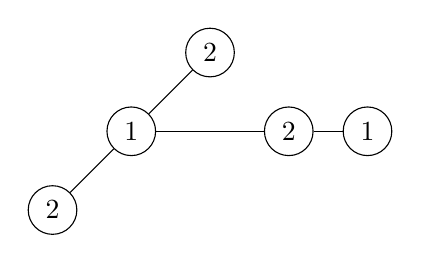
\begin{tikzpicture}

% Noeuds
\node[circle, draw] (A) at (0,0) {1};
\node[circle, draw] (B) at (1,1) {2};
\node[circle, draw] (C) at (-1,-1) {2};
\node[circle, draw] (D) at (2,0) {2};
\node[circle, draw] (E) at (3,0) {1};

% Arêtes
\draw (A) -- (B);
\draw (A) -- (C);
\draw (A) -- (D);
\draw (D) -- (E);

\end{tikzpicture}

Le nombre minimal de couleurs utilisées est noté \( m \). La coloration 
minimale pour le graphe ci-haut est donc $m = 2$.

Pour modéliser ce problème, on utilise deux types de variables binaires :
\begin{align*}
&c_i =
\begin{cases}
1 & \text{si la couleur \( i \) est utilisée} \\
0 & \text{sinon}
\end{cases}
\\
&x_{ij} =
\begin{cases}
1 & \text{si le sommet \( j \) est coloré avec \( i \)} \\
0 & \text{sinon}
\end{cases}
\end{align*}

L'objectif est de minimiser \( \sum_{i=1}^{m} c_i \), tout en respectant les 
contraintes suivantes :
\[
\boxed{
x_{ij} + x_{ik} \leq 1 \quad \text{pour tout couple de sommets adjacents} \ (j, k)
}
\]
\[
\sum_{i=1}^{m} x_{ij} = 1 \quad \text{pour tout sommet} \ j
\]
où \( c_i \in \{0, 1\} \) et \( x_{ij} \in \{0, 1\} \).

\section{Deux principes généraux en PLNE}

Soit un problème \( P \) et sa relaxation continue \( \tilde{P} \), où les 
contraintes d'intégralité sont relâchées. Nous avons alors :
\[
F(P) \subseteq F(\tilde{P}) \quad \text{et} \quad v(\tilde{P}) \leq v(P)
\]
Les principes suivants s'appliquent :
\begin{enumerate}
    \item Si \( F(P) \subseteq F(\tilde{P}) \), alors la valeur optimale de 
    \( \tilde{P} \) est toujours meilleure ou égale à celle de \( P \).
    
    \item Si \( x^* \) est une solution optimale entière de \( \tilde{P} \), 
    alors \( x^* \) est aussi solution optimale de \( P \).
\end{enumerate}

\section{Exemple : Problème de relaxation continue}

Considérons un problème \( P \) et sa relaxation continue \( \tilde{P} \) avec 
les contraintes suivantes :
\[
P: \quad \text{Minimiser} \quad z = -x_1 - 5x_2
\]
\[
\text{s.a.} \quad x_1 + 10x_2 \leq 20, \quad x_1 \leq 2, \quad x_1, x_2 \geq 0
\]
Dans la relaxation \( \tilde{P} \), les variables \( x_1 \) et \( x_2 \) ne sont 
plus contraintes à être entières. La solution fractionnaire est donnée par :
\[
x_1 = 2, \quad x_2 = 9/5
\]
Cependant, la solution entière optimale est obtenue par des algorithmes de PLNE, 
car ni l'arrondi ni la troncature ne donnent des solutions optimales dans ce cas.


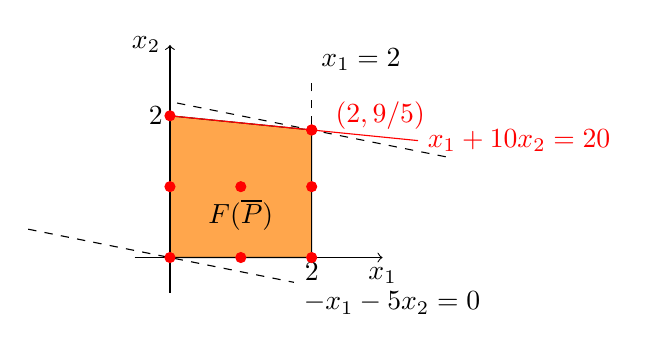
\begin{tikzpicture}[scale=0.9]

% Coloration de la région
\filldraw[fill=orange, fill opacity=0.7] (0,0) -- (2,0) -- (2,1.8) -- (0,2) -- cycle;

% Axes
\draw[->] (-0.5,0) -- (3,0) node[below] {$x_1$};
\draw[->] (0,-0.5) -- (0,3) node[left] {$x_2$};

% Étiquettes des axes
\node at (2,-0.2) {2};
\node at (-0.2,2) {2};

% Les lignes contraintes
\draw[dashed] (-2,0.4) -- (1.75,-0.35) node[below right] {$-x_1 - 5x_2 = 0$};
\draw[dashed] (2,0) -- (2,2.5) node[above right] {$x_1 = 2$};
\draw[dashed] (.1,2.18) -- (4, 1.4); 
\draw[red] (0,2) -- (3.5, 1.65) node[right] {$x_1 + 10x_2 = 20$};
% Les points
\filldraw[red] (2,1.8) circle (2pt);
\filldraw[red] (1,1) circle (2pt);
\filldraw[red] (0,1) circle (2pt);
\filldraw[red] (1,0) circle (2pt);
\filldraw[red] (2,1) circle (2pt);
\filldraw[red] (0,2) circle (2pt);
\filldraw[red] (0,0) circle (2pt);
\filldraw[red] (2,0) circle (2pt);
\filldraw[red] (2,9/5) circle (2pt);

% Légende point (2,9/5)
\node[right] at (2.2,10/5) {\textcolor{red}{$(2,9/5)$}};

% Le label de F(\overline{P})
\node at (1,0.6) {\textcolor{black}{$F(\overline{P})$}};

\end{tikzpicture}

\chapter{Algorithme Branch and Bound}

\section{Introduction}

L'algorithme de \textbf{Branch-and-Bound} est utilisé pour résoudre des 
problèmes de \textbf{programmation linéaire en nombres entiers}. Il divise un 
problème en sous-problèmes tout en exploitant les solutions fractionnaires et 
entières.

\section{Branchement}

Si la solution optimale de la relaxation continue \( \overline{P} \) est 
fractionnaire, le problème est divisé en deux sous-problèmes \( P_1 \) et 
\( P_2 \) tels que :
\[
F(P_1) \cap F(P_2) = \emptyset, \quad F(P_1) \cup F(P_2) = F(P)
\]
Cela permet de réduire les domaines des sous-problèmes :
\[
F(\overline{P}_1) \subset F(\overline{P}), \quad F(\overline{P}_2) \subset F(\overline{P})
\]

\section{Évaluation des sous-problèmes}

L'algorithme explore les sous-problèmes en suivant un parcours en profondeur. La 
solution optimale entière trouvée est utilisée pour mettre à jour la borne 
supérieure \( \overline{z} \).

La relaxation continue \( \overline{P} \) fournit une borne inférieure \( z \). Si un 
sous-problème produit une meilleure solution entière, la borne supérieure est 
mise à jour.

\section{Critère d'arrêt}

Le processus de division s'arrête pour un sous-problème \( P_C \) si :
\begin{itemize}
    \item Le domaine réalisable est vide.
    \item La solution optimale de \( P_C \) est entière.
    \item La solution optimale fractionnaire de \( P_C \) est telle que 
    \( v(P_C) \geq \overline{z} \).
\end{itemize}

Dans ces cas, diviser \( P_C \) ne permet pas de trouver une meilleure solution.

\section{Branchement et Pseudo-Code}

Si la solution optimale \( \overline{x} \) de \( P_C \) est fractionnaire, on choisit 
une variable \( x_j \) ayant une valeur fractionnaire \( w \). Deux sous-problèmes 
sont alors créés :
\[
P_{C_1} : x_j \leq \lfloor w \rfloor, \quad P_{C_2} : x_j \geq \lceil w \rceil
\]





\begin{algorithm}[H]
\caption{Branch-and-Bound}
\SetAlgoLined
Étape 0 : Initialiser \( L \leftarrow \emptyset \), \( \overline{z} \leftarrow \infty \),
\( x^* \leftarrow \emptyset \)\;
Étape 1 : Résoudre \( \overline{P} \), obtenir \( x^* \)\;
\If{ \( x^* \) est entier }{
    Aller à l'étape 3\;
}
\Else{
    Diviser \( P \) en \( P_1 \) et \( P_2 \), ajouter à \( L \)\;
}
Étape 2 : Pour chaque sous-problème dans \( L \), résoudre \( P_C \)\;
\If{ \( F(P_C) = \emptyset \) \textbf{ou} \( v(P_C) \geq \overline{z} \)}{
    Continuer\;
}
\ElseIf{ \( x^* \) est entier \textbf{et} \( v(P_C) < \overline{z} \)}{
    Mettre à jour \( \overline{z} \) et \( x^* \)\;
}
\Else{
    Diviser \( P_C \)\;
}
Étape 3 : Retourner \( x^* \)\;
\end{algorithm}



\end{multicols*}
\end{document}
